\setcounter{chapter}{2}
\chapter{Il Formalismo Lagrangiano}

\section{Introduzione}

Consideriamo un sistema costituito da due punti materiali giacenti nel piano (x,z), rispettivamente $P_1(x_1,z_1)$ e $P_2(x_2,z_2)$. La particella $P_1$ \`{e} vincolata a muoversi su una circonferenza di raggio R, mentre $P_2$ sull'asse delle ordinate, inoltre i due punti sono legati tra loro da un'asta inestensibile ed ideale di lunghezza d. Sul sistema agisce la forza di gravit\`{a}.

 
\begin{figure}[ht]
\vspace{0.2in}
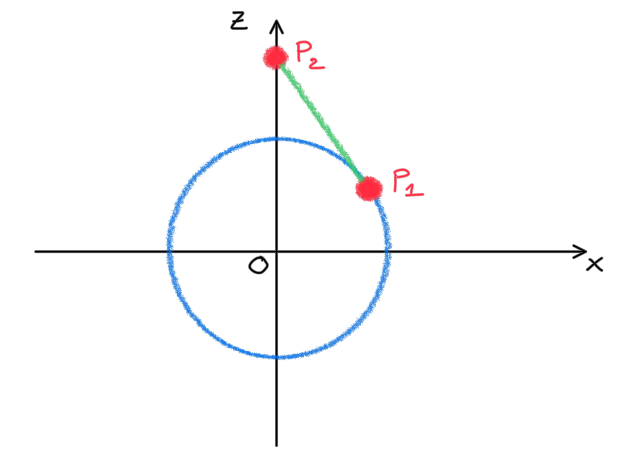
\includegraphics[width = 11.5cm]{vincolo}	
\centering
\end{figure}

\noindent I vincoli sui punti materiali sono rispettivamente rappresentabili dalle seguenti equazioni
\begin{align}
	\left \{ \begin{array}{l}
		x_{1}^2 + x_{2}^2 - R^2 = 0 \\
		x_2 = 0\\
		(x_1 - x_2)^2 + (z_1 - z_2)^2 - d^2 = 0
	\end{array} \right.
\end{align}
se vogliamo descrivere la dinamica delle singole particelle utilizzando gli strumenti della meccanica Newtoniana otteniamo per ciascuna particella un sistema di due equazioni 
\begin{align}
	\left \{ \begin{array}{l}
		m_1 \ddot{\bm{x}_1} = \bm{F}_{x_1}^{tot} \\
		m_1 \ddot{\bm{z}_1} = \bm{F}_{z_1}^{tot}
	\end{array} \right.
\end{align}
dove la forza totale agente sulla particella $P_{1}$ lungo uno degli assi pu\`{o} essere scritta come la somma di due grandezze
\begin{equation}
	\bm{F}_{x_1}^{tot} = \bm{F}^{attive}_1 + \bm{\phi}_1
\end{equation}
che rappresentano rispettivamente le forze che siamo in grado d'identificare e che agiscono sulla particella definendone lo stato di moto e le forze che prendono il nome di \textit{reazione vincolare} e definiscono i vincoli che limitano lo stato di moto della particella lungo determinate traiettorie e sono forze che non sono conosciute a priori. Le reazioni vincolari possono essere determinate esplicitamente solo quando si sono risolte le equazioni del moto.

\subsection*{Esempio - Il Pendolo Semplice}

Consideriamo un pendolo semplice in un piano (x,y) costituito da un filo inestensibile ed ideale di lunghezza L fissato nell'origine O del sistema e alla cui estremit\`{a} \`{e} presente un punto materiale P(x,y) di massa \textit{m}. La particella \`{e} sogetta alla forza di gravit\`{a}.
\newline 

\noindent Il vincolo sulla particella P \`{e} rappresentato dall'espressione 
\begin{equation*}
	x^2+y^2 - L^2 = 0
\end{equation*}
Le equazioni del moto sono date dal sistema 

\begin{figure}[!ht]
\centering
\begin{minipage}{.5\textwidth}
  \centering
  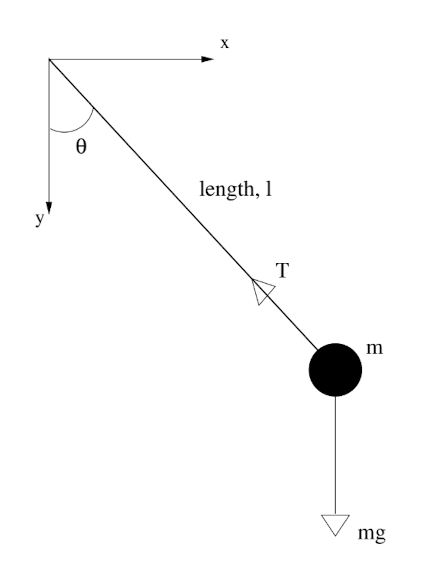
\includegraphics[width=.7\linewidth]{pendolo}
\end{minipage}%
\begin{minipage}{.5\textwidth}
 	\begin{align*}
 		\left \{ \begin{array}{l}
 			 m\ddot{x} = - T_{x}/L \\[0.1in]
 			 m\ddot{y} = mg - T_y/L
 		\end{array} \right.
 	\end{align*}
\end{minipage}
\end{figure}
dove \textbf{T} rappresenta la tensione e la reazione vincolare del sistema che non conosciamo a priori, ma la sua determinazione dipende dalle soluzioni del sistema. Infatti parametrizzando il vincolo in coordinate polari 
	\begin{align*}
 		\left \{ \begin{array}{l}
 			 x = Lcos\theta\\[0.1in]
 			 y = Lsin\theta
 		\end{array} \right.
 	\end{align*}
si ha che la soluzione delle equazioni del moto \`{e} data da 
\begin{equation*}
	\ddot{\theta} = - (g/L)sin\theta 
\end{equation*} 
e sostituendo nelle equazioni del sistema si ha che la reazioni vincolare costituita dalla tensione \`{e} data da 
\begin{equation*}
	T=m l \dot{\theta}^2+m g \cos \theta
\end{equation*}
Nel caso di sistemi molto complessi il calcolo delle reazioni vincolari non risulta essere agevole da un punto di vista computazionale. Ci chiediamo dunque se esista un modo per evitarne il calcolo, ma che tenga conto dell'informazione che fornisce. Per questo motivo ed altri s'introduce la meccanica Lagrangiana, che mediante lo studio delle equazioni di E-L permette di determinare le soluzione del moto incorporando le informazioni delle condizioni di vincolo.

\section{Vincoli Posizionali}

Gli esempi visti nell'introduzione ci suggeriscono che un vincolo \`{e} una condizione che limita i possibili valori che possono assumere le coordinate. Supponiamo di avere N punti materiali in uno spazio 3D e consideriamo la posizione di tutti i punti in unico vettore 
$\bm{x} = (x_1,.....,x_{3N})$.

\begin{definition}
	 Definiamo vincolo una funzione f che lega tra di loro le coordinate dei punti.
\end{definition}
\noindent I vincoli si dividono in due macro categorie:
\begin{itemize}
	\item \textbf{Vincoli Olonomi}: la funzione $f(\bm{x},t)$ di vincolo dipende solo dalla posizione $\bm{x}$ .
	\item \textbf{Vincoli Anolonomi}:la funzione $f(\bm{x},\dot{\bm{x}},t)$ di vincolo dipende sia dalla posizione $\bm{x}$ che dalla velocit\`{a} $\dot{\bm{x}}$.
\end{itemize}

\begin{definition}
	Si definisce bilatero un vincolo olonomo f tale per cui 
	\begin{equation}
		f(\bm{x},t) = 0
	\end{equation}
\end{definition}
\begin{definition}
	Sia f una funzione di vincolo tale che 
	\begin{equation}
		f(\bm{x},\dot{\bm{x}},t) \geq 0
	\end{equation}
allora f \`{e} un vincolo unilatero e anolonomo per la disuguaglianza in senso stretto.
\end{definition}

\begin{definition}
	Per un vincolo f dipende dal tempo si aggiunge il suffisso mobile.
\end{definition}

\subsection{Gradi di Libert\`{a}}
Consideriamo un sistema di N punti materiali i cui punti sono soggetti a k vincoli posizionali.

\begin{equation}
\left\{\begin{array}{l}
f_1(\underline{x})=0 \\
f_2(\underline{x})=0 \\
\;\;\;\vdots \\
f_k(\underline{x})=0
\end{array}\right.
\end{equation}
I vincoli ci permettono di legare tra di loro le coordinate dei punti, in modo da esplicitarle l'una rispetto all'altra, in questo modo si abbassa la dimensione del problema. Come si \`{e} visto nell'esempio del pendolo anche la parametrizzazione dei vincoli permette di ridurre le dimensioni del problema, in particolare in quel caso si \`{e} passati da 2 coordinate (x,y) ad una sola data dall'angolo $\theta$.

\begin{definition}
	Dato un sistema di N particelle nello spazio servono 3N coordinate per descrivere il sistema , se queste sono legate tra loro da k relazioni di vincolo la dimensione del problema \`{e} riducibile 3N-k gradi di libert\`{a}.
\end{definition}

\begin{remark}
 Il sistema dei k vincoli olonomi in uno spazio $\mathbb{R}^{3N}$ identifica un sottoinsieme(variet\`{a} differenziabile) che pu\`{o} essere parametrizzata da 3N-k variabili.	
\end{remark}

\subsection{Cambi di Coordinate}
La parametrizzazione di un vincolo \`{e} una trasformazione di coordinate locale, per superfici generiche \`{e} necessario definire diverse parametrizzazioni che prendono il nome di carte e nei punti in cui si sovrappongono devono essere compatibili.

\begin{definition}
	Una trasformazione di coordinate \`{e} una funzione vettoriale regolare e biunivoca $\bm{\varphi} : U \subseteq \mathbb{R}^m \rightarrow \mathbb{R}^n$ dove $0< m \leq n$ che definisce un sistema di n equazioni  
\begin{align}
\left \{ \begin{array}{l}
 x_1=\varphi_1\left(q_1, \ldots, q_m\right) \\
 \quad \quad \vdots \\
 x_n=\varphi_n\left(q_1, \ldots, q_m\right)
\end{array} \right.
\end{align}
\end{definition}
Il sistema di funzioni definito in (3.7) rappresenta un pezzo di superficie M = $\bm{\varphi}(U) \subset \mathbb{R}^n$ di dimensione m che giace in $\mathbb{R}^n$.
Affinch\`{e} la trasformazioni di coordinate sia biettiva \`{e} necessario che il determinante della matrice Jacobiana associato sia non nullo.

\begin{definition}
	Se consideriamo le coordinate locali $(q_1,...,q_m)$ e le fissiamo tutte eccetto una otteniamo una curva nello spazio delle $(x_1,...,x_n)$ poich\`{e} dipendono da una sola coordinata. Tale curva prende il nome di \textit{linea coordianta}.
\end{definition}

\begin{figure}[!ht]
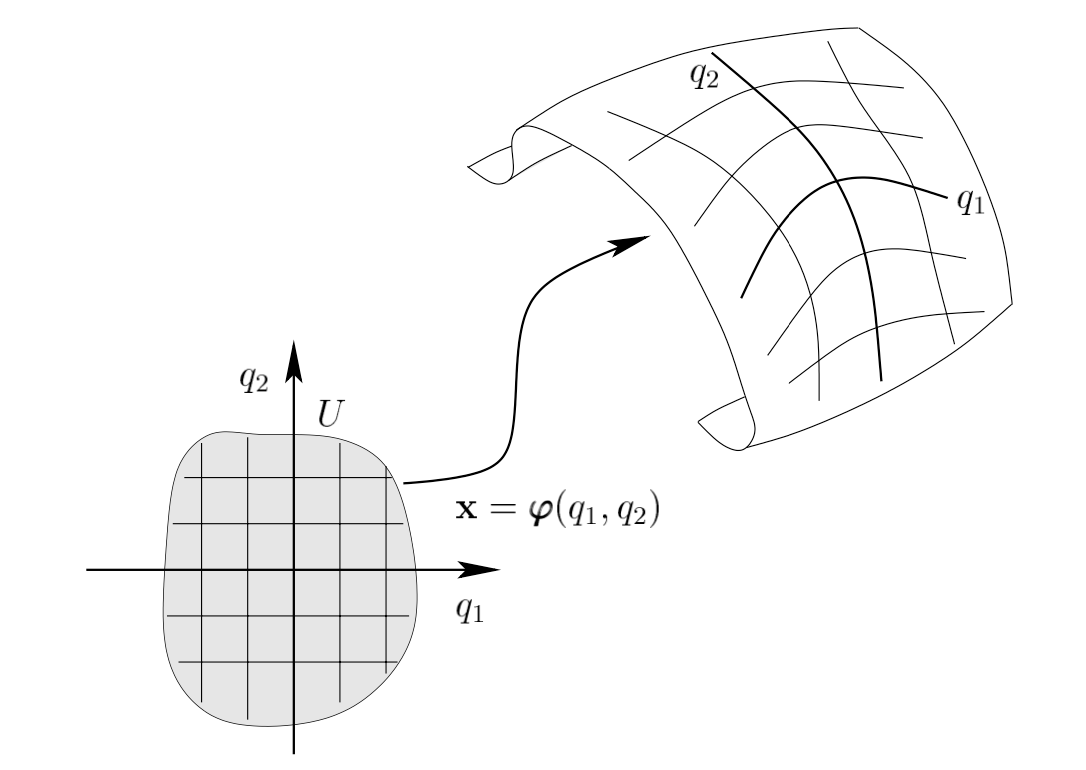
\includegraphics[scale = 0.5]{linee}	
\centering
\end{figure}

\begin{definition}
	Le coordinate $(q_1,...,q_m)$ vengono definite \textit{coordinate libere} poich\`{e} non esistono relazioni di vincolo tra di esse.
\end{definition}

\noindent Variando ciascuna coordinata $q_j$ si ottengono diverse linee coordinate che rappresentano le possibili traiettorie compatibili con il vincolo. Come sono fatte le velocit\`{a} compatibili ?

\subsection{Velocit\`{a} generalizzate (o virtuali)}

Consideriamo un punto della superficie M identificato dalle coordinate libere $(q_1,...,q_m) \in U$ e supponiamo di far variare solo la coordinata $q_j$ e di tenere fisse le altre. Ipotizzando una variazione infinitesima h definiamo il rapporto incrementale 
\begin{equation}
\lim _{h \rightarrow 0} \frac{\mathbf{x}\left(q_1, \ldots, q_j+h, \ldots, q_m\right)-\mathbf{x}\left(q_1, \ldots, q_j, \ldots, q_m\right)}{h}=\frac{\partial \mathbf{x}}{\partial q_j}
\end{equation}
L'esistenza del limite \`{e} assicurata dalla ipotesi di regolarit\`{a} delle funzioni, posta inizialmente. La quantit\`{a} $\frac{\partial \bm{x}}{\partial q_j}$ \`{e} un vettore in $\mathbb{R}^n$ applicato nel punto $\bm{x}(q_1,...,q_m)$ e che per costruzione \`{e} tangente alla linea coordinata definita da $q_j$ e dunque alla superficie M. Reiterando il procedimento si costruisce un insieme di m vettori 
\begin{equation}
\left\{\frac{\partial \mathbf{x}}{\partial q_1}, \ldots, \frac{\partial \mathbf{x}}{\partial q_m}\right\}
\end{equation}
tangenti alla superficie M. Il fatto che lo Jacobiano associato alla trasformazione di coordinate abbia rango massimo, fa si che i vettori siano linearmente indipendenti, e quindi si intersechino trasversalmente nel punto $\bm{x}(q_1,...,q_m)$. Le linee coordinate definite sulla superficie non sono in questo modo tangenti tra loro.
L'insieme di vettori definiti in (3.9) costituisce una base locale per lo spazio vettoriale dato da un piano tangente alla superficie M di dimensione m passante per il punto $\bm{x}(q_1,...,q_m)$. Tale spazio prende il nome di \textbf{spazio tangente} e si denota con $T_{x}M$.
Ovviamente la base dipende dalla scelta delle coordinate locale $q_1,...,q_m$.

\begin{figure}[!ht]
\vspace{0.1in}
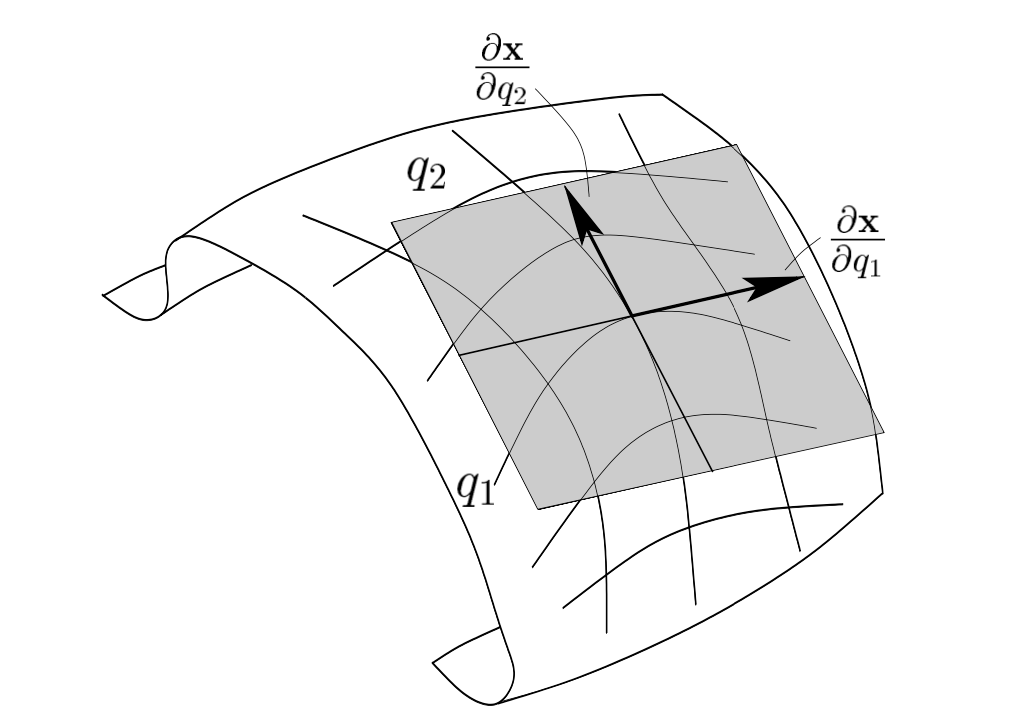
\includegraphics[scale = 0.5]{base}	
\centering
\end{figure}

Consideriamo le coordinate generalizzate $q_1(t),...,q_{m}(t)$ come funzioni dipendenti dal tempo, per $t \in \mathcal{F} \subset \mathbb{R}$ intervallo aperto, scelto in modo che la sua immagine non esca dalla carta U. In questo modo otteniamo una tratto di curva in U, dove sono definite le coordinate generalizzate, che mediante la mappa $\bm{x} = \bm{\varphi}(q_1,...q_m)$ genera una curva sulla superficie.
\newpage
\begin{figure}[!ht]
\vspace{0.1in}
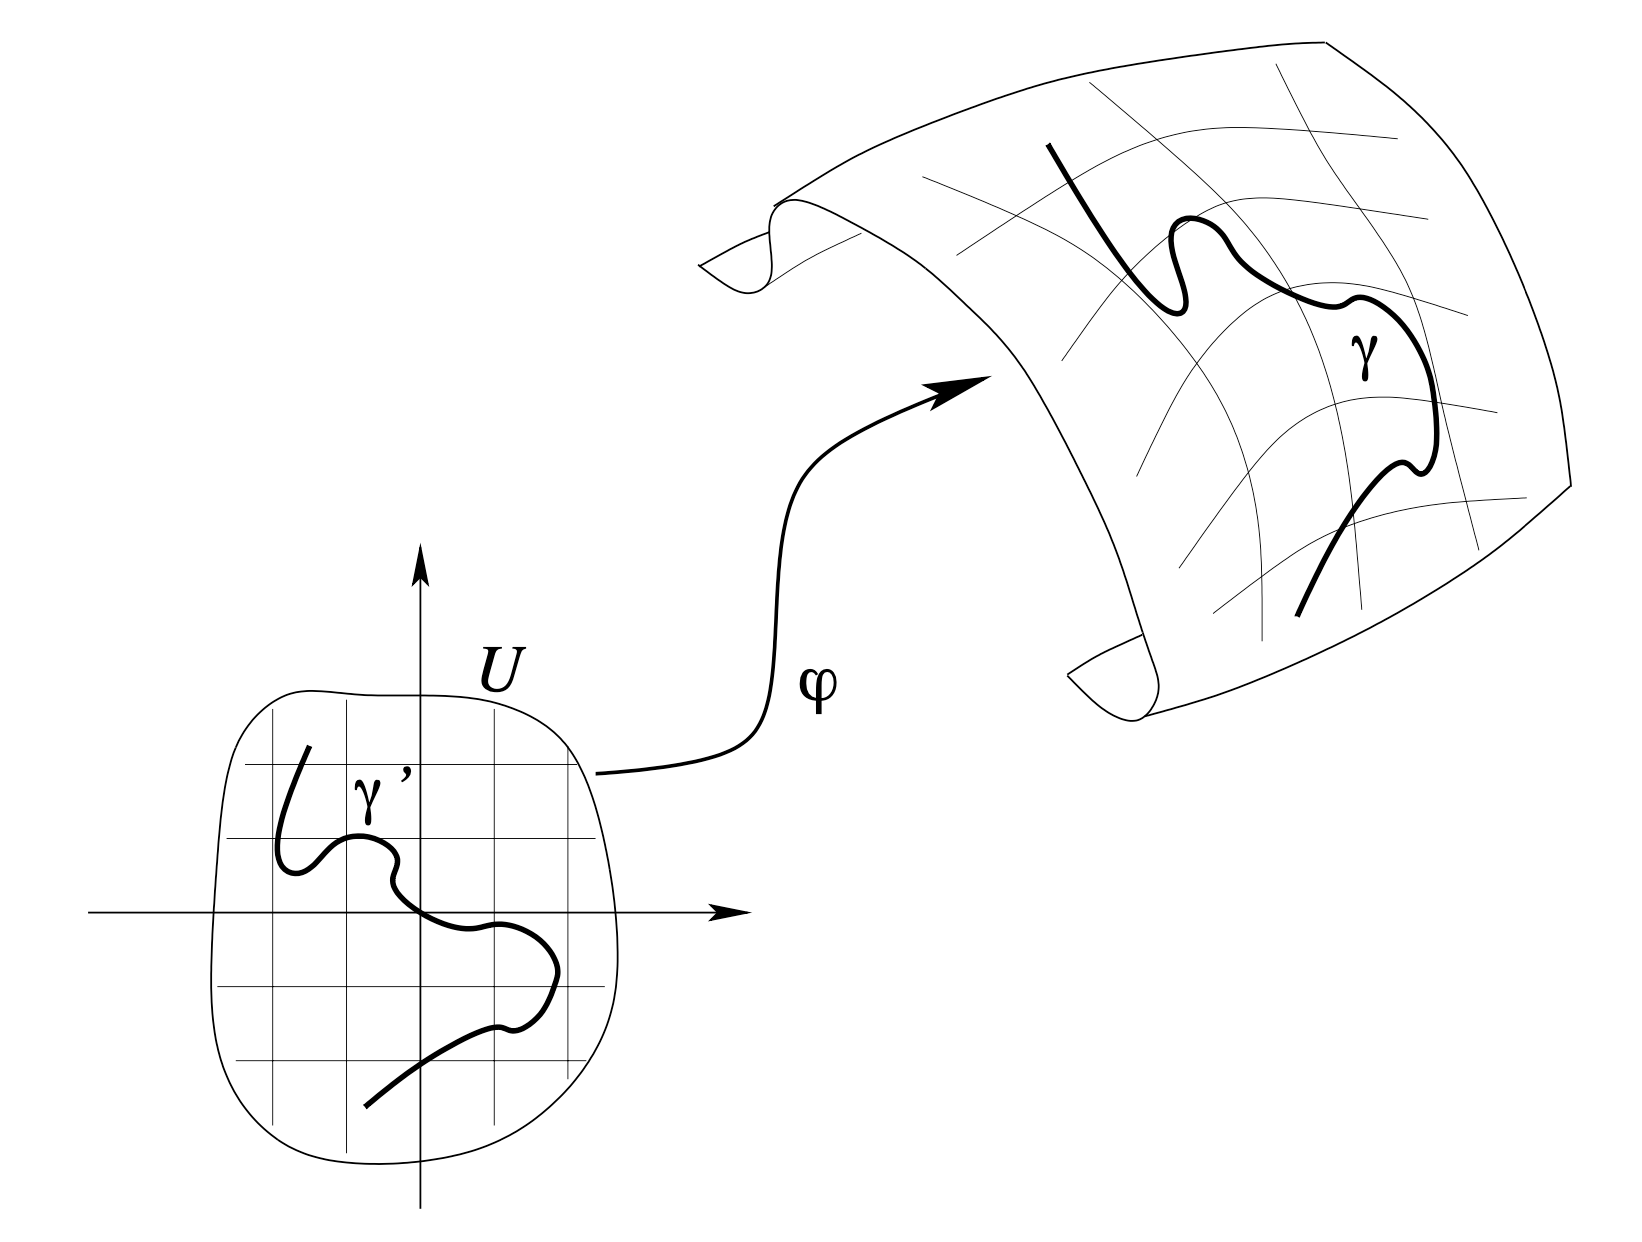
\includegraphics[scale = 0.4]{map}	
\centering
\end{figure}
La curva cos\`{i} ottenuta la indicheremo con $\bm{x}(t) : \mathcal{F} 
\rightarrow U \subset \mathbb{R}^n$. Definiamo $\bm{x}(t_0) = \bm{x}_0$ il valore delle coordinate nell'istante di tempo $t_0 \in \mathcal{F}$ rispetto al quale calcoliamo il rapporto incrementale per uno spostamento infinitesimo h
\begin{equation}
\bm{\dot{x}}\left(t_0\right)=\lim _{h \rightarrow 0} \frac{\mathbf{x}\left(t_0+h\right)-\mathbf{x}\left(t_0\right)}{h} = \frac{d \bm{x}(t)}{dt}\Big \vert_{t = t_0}
\end{equation}
poich\`{e} $\bm{x}$ dipende dalle coordinate generalizzate che dipendono dal tempo abbiamo che la relazione (3.10) \`{e} riscrivibile come
\begin{equation}
	\bm{\dot{x}}\left(t_0\right) = \frac{d \bm{x}(t)}{dt}\Big \vert_{t = t_0} = \sum_{j=1}^{m}\frac{\partial \bm{x}}{\partial q_j}\dot{q_j}\Big \vert_{t=t_0}
\end{equation}
dunque $\dot{\bm{x}}(t_0)$ \`{e} un vettore tangente alla superficie M nel punto $\bm{x}_0$ e le sue componenti rispetto alla base dello spazio tangente sono $\dot{q}_j(t_0)$. Le variabili $\dot{q}_1,...,\dot{q}_{m}$ prendono il nome di \textbf{velocit\`{a} generalizzate}.

\begin{remark}
Le velocit\`{a} generalizzate in (3.11) definiscono un sistema di equazioni differenziali del primo ordine.	
\end{remark}

\section{Equazioni di Eulero-Lagrange come equazioni di bilancio energetico}

Consideriamo un punto materiale P definito in uno spazio 3D vincolato a muoversi lungo una curva, effettuiamo una parametrizzazione del vincolo e definiamo una trasformazione biunivoca e regolare delle coordinate di partenza
\begin{equation}
	\bm{x}(q) = [x(q),y(q),z(q)]
\end{equation}
le velocit\`{a} compatibili con il vincolo saranno date dal vettore 
\begin{equation}
	\dot{\bm{x}}(t) = \Big [\frac{dx(q)}{dt}\dot{q},\frac{dy(q)}{dt}\dot{q},\frac{dz(q)}{dt}\dot{q} \Big ]
\end{equation}
Assumiamo inoltre che l'evoluzione dinamica della particella sia dovuta all'azione di una forza attiva conservativa $\bm{F}^{attiva} = [F_x,F_y,F_z] = - \nabla U(x,y,z)$.
La potenza delle forze attive $\pi^{attive} = \bm{F}^{attive} \cdot \dot{\bm{x}}$ \`{e} riscrivibile rispetto alle coordinate di vincolo come 
\begin{align}
\pi^{\text {attive}}=\left[-\frac{\partial U}{\partial x},-\frac{\partial U}{\partial y},-\frac{\partial U}{\partial z}\right]\cdot\left[\frac{dx(q)}{dq},\frac{dy(q)}{dq},\frac{dz(q)}{dq}\right] \dot{q} = \\[0.2in]
= -\left[\frac{\partial U}{\partial x} \frac{d x}{d q}+\frac{\partial U}{\partial y} \frac{d y}{d q}+\frac{\partial U}{\partial z} \frac{d z}{d q}\right] \dot{q} = - \frac{dU}{dq} \cdot \dot{q}
\end{align}
Definiamo l'energia cinetica del sistema rispetto alle coordinate generalizzate come
\begin{equation}
	K(q,\dot{q}) = \frac{1}{2} m \Big [ (x^{\prime})^2 + (y^{\prime})^2 + (z^{\prime})^2 \Big] \dot{q}^2 = \frac{1}{2} G(q)\dot{q}^2 
\end{equation}
dove G(q) per sistemi a pi\`{u} di una dimensione prende il nome di matrice dell'energia cinetica. Si osservi che G(q) dipende solo dalle coordinate generalizzate. \`{E} definita strettamente positiva $G(q) > 0$, ovvero non si annulla mai poich\`{e} se fosse uguale a 0, vorebbe dire che la matrice Jacobiana associata alla parametrizzazione del vincolo non ha rango massimo e dunque non si avrebbe una trasformazione di coordinate.
La potenza totale \`{e} definita come derivata totale rispetto al tempo dell'energia cinetica
\begin{equation}
	\pi ^{totale} = \frac{dK(q,\dot{q})}{dt} = \frac{\partial K}{\partial q}\dot{q} + \underbrace{\frac{\partial K}{\partial\dot{q}}}_{\textcolor{red}{A}} \underbrace{\frac{d \dot{q}}{dt}}_{\textcolor{red}{\dot{B}}}=
\end{equation}
possiamo riscrivere il secondo addendo utilizzando la relazione
\begin{equation*}
	\textcolor{red}{A\dot{B} = \frac{d(AB)}{dt} - \dot{A}B} 
\end{equation*}
e dunque la (3.17) diventa 
\begin{equation*}
=\frac{\partial K}{\partial q} \dot{q}+\frac{d}{d t}\left(\frac{\partial K}{\partial \dot{q}} \dot{q}\right)-\left[\frac{d}{d t}\left(\frac{\partial K}{\partial \dot{q}}\right)\right] \dot{q}=
\end{equation*}
\begin{equation}
=\dot{q}\left[\frac{\partial k}{\partial q}-\frac{d}{d t}\left(\frac{\partial K}{\partial \dot{q}}\right)\right]+\frac{d}{d t} \underbrace{\left(\frac{\partial K}{\partial \dot{q}} \dot{q}\right)}_{\textcolor{red}{C}}=
\end{equation}
dove il termine C per un sistema ad un grado di libert\`{a} \`{e} dato da 
\begin{equation}
	\frac{\partial K}{\partial \dot{q}}\dot{q} = G(q)\dot{q}^2 = 2K(q,\dot{q})
\end{equation}
sostituendo in 3.18 si ha 
\begin{equation}
=\dot{q}\left[\frac{\partial K}{\partial q}-\frac{d}{d t}\left(\frac{\partial K}{\partial \dot{q}}\right)\right]+2 \frac{d}{d t} K(q, \dot{q})
\end{equation}
di conseguenza la potenza totale rispetto alle coordinate e velocit\`{a} generalizzate \`{e} data da 
\begin{equation}
\frac{d}{d t} K(q, \dot{q})=\left[\frac{d}{d t}\left(\frac{\partial K}{\partial \dot{q}}\right)-\frac{\partial K}{\partial q}\right] \dot{q}
\end{equation}
il termine di sinitra della 3.20 pu\`{o} essere riscritto come 
\begin{equation}
	\pi^{totale} = \frac{dK(q,\dot{q})}{dt} = \bm{F}^{totali} \cdot \dot{\bm{x}}
\end{equation}
come abbiamo visto nel capitolo della meccanica Newtnonia le forze totali possono essere riscritte come il contributo di forze attive e forze vincolari $\bm{F}^{totali} = \bm{F}^{attive} + \bm{\phi}_{vincolo}$.
Per collegare l'equazione (3.21) all'equazione (3.15) abbiamo bisogno di formulare l'ipotesi che i vincoli siano lisci.
\begin{definition}
	Si definisce una forza di vincolo $\bm{\phi}$ liscia se la sua potenza \`{e} nulla lungo le posizioni e velocit\`{a} compatibili con il vincolo.
\begin{equation}
	\pi^{vincoli} = \bm{\phi}_{vincoli} \cdot \bm{\dot{x}} = 0 
\end{equation}
\end{definition}
\noindent Sotto tale ipotesi abbiamo che 
\begin{equation}
-\frac{d U}{d q} =\left[\frac{d}{d t}\left(\frac{\partial K}{\partial \dot{q}}\right)-\frac{\partial K}{\partial q}\right]
\end{equation}
poich\`{e} il potenziale U dipende solo dalle coordinate generali di posizione possiamo riscrivere l'equazione 3.23 come
\begin{equation}
\frac{d}{d t} \Big [\frac{\partial (K-U)}{\partial \dot{q}} \Big ]=\frac{\partial(K-U)}{\partial q}
\end{equation}
La grandezza K-U prende il nome di funzione \textbf{Lagrangiana} del sistema
\begin{equation}
	\mathcal{L}(q,\dot{q}) = K(q,\dot{q}) - U(q)
\end{equation}
riscrivendo l'equazione 3.24 rispetto alla Lagrangiana si ottiene \textbf{l'equazione di Eulero-Lagrange}
\setlength\fboxsep{0.15in}
\begin{equation}
\boxed{\frac{d}{d t}\left[\frac{\partial}{\partial \dot{q}} \mathcal{L}(q, \dot{q})\right]=\frac{\partial}{\partial q} \mathcal{L}(q, \dot{q})}
\end{equation}
e definisce le equazioni del moto per le coordinate generalizzate.
\begin{remark}
L'equazione 3.23 pu\`{o} essere definita anche se le forze non sono di natura conservativa.	
\end{remark}

\section{L'energia del sistema come costante del moto sotto l'ipotesi di vincolo liscio (Integrale di Jacobi) }
Si consideri una Lagrangiana $\mathcal{L}(q,\dot{q})$ non dipendente esplicitamente dal tempo, ovvero $\frac{\partial \mathcal{L}}{\partial t} = 0$. Calcoliamo la derivata totale della Lagrangiana rispetto al tempo
\begin{equation}
\begin{aligned}
\frac{d}{d t}[\mathcal{L}(q, \dot{q})]= & \frac{\partial \mathcal{L}}{\partial q} \dot{q}+\frac{\partial \mathcal{L}}{\partial \dot{q}} \frac{d \dot{q}}{d t} = & \\[0.1in]
= & \dot{q} \left[\frac{\partial \mathcal{L}}{\partial q}-\frac{d}{d t} \frac{\partial \mathcal{L}}{\partial \dot{q}}\right]+\frac{d}{d t}\left[\frac{\partial \mathcal{L}}{\partial \dot{q}} \dot{q}\right] \\
\end{aligned}
\end{equation}
scelta una soluzione q(t) soluzione delle equazioni di Eulero-Lagrange l'addendo si sinistra \`{e} nullo. Dunque possiamo riscrivere la 3.27 come
\begin{equation}
\frac{d}{d t}\left[\frac{\partial \mathcal{L}}{\partial q} \dot{q}-\mathcal{L}\right] = 0
\end{equation}
di conseguenza la grandezza $\frac{\partial \mathcal{L}}{\partial q} \dot{q}-\mathcal{L}$ \`{e} una costante del moto e prende il nome di \textbf{integrale di Jacobi}. Utilizzando la relazione 3.19 possiamo riscrivere la costante del moto come
\begin{equation}
\frac{\partial \mathcal{L}}{\partial \dot{q}} \dot{q}-\mathcal{L}=2 K-\mathcal{L}=K+U = E
\end{equation}
di conseguenza l'energia totale del sistema \`{e} una costante del moto.
\section{Vincoli Anolonomi}
Consideriamo un punto materiale vincolato a muoversi lungo una circonferenza di raggio R, in una configurazione di questo tipo velocit\`{a} e posizione sono ortogonali tra loro.
\begin{equation}
	2(x\dot{x} + y \dot{y}) = 0 \iff <\bm{x},\bm{\dot{x}}> =0
\end{equation}
ogni volta che \`{e} possibile riscrivere un vincolo rispetto alle coordinate laplaciane questo prende il nome di vincolo Olonomo, esistono per\`{o} condizioni doce non \`{e} possibile scrivere i vincoli sulle velocit\`{a} rispetto alle posizioni, tale tipologia di vincoli prendomo il nome di \textbf{anolonomi}.
\subsubsection{Esempio}

Consideriamo un sistema dato da due ingranaggi di raggio $R_1$ e $R_2$ dove $R_2 > R_1$ collegati da una catena.

\begin{wrapfigure}{r}{0.5\textwidth}
  \begin{center}
    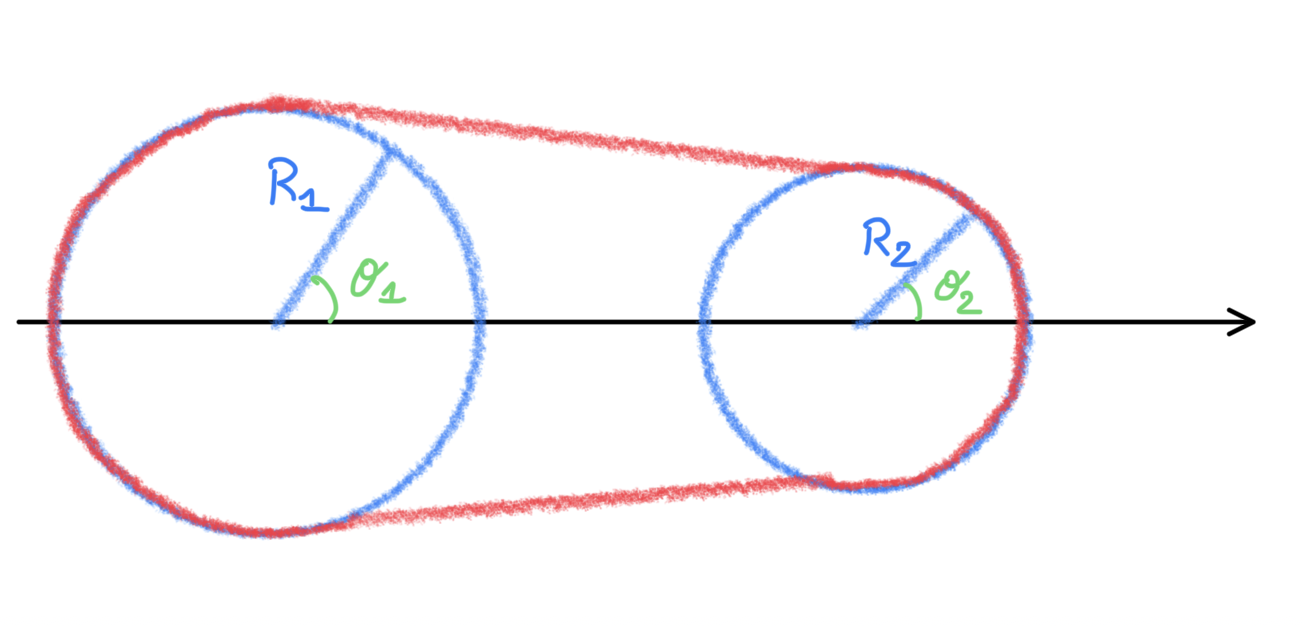
\includegraphics[width=0.48\textwidth]{catena}
  \end{center}
\end{wrapfigure}
La configurazione della circonferenza di raggio $R_1$ e $R_2$ \`{e} identificata dai rispettiva angoli $\theta_1$ e $\theta_2$. Essendo i due ingranaggi legati da una catena avremo che le rispettive velocit\`{a} dei singoli ingranaggi devono coincidere dunque 
\begin{equation*}
	R_1 \dot{\theta}_{1} = R_2 \dot{\theta}_{2}
\end{equation*}
che equivale alla condizione di vincolo
\begin{equation*}
	\frac{d}{dt}(R_1 \theta_1 - R_2 \theta_2) = 0 
\end{equation*}
dalla relazione precedente sappiamo che per ogni tempo t gli angoli che possono essere assunti non sono qualsiasi ma devono soddisfare la condizione 
\begin{equation*}
	R_1\theta_1 - R_2 \theta_2 = C
\end{equation*}
di conseguenza il vincolo \`{e} olonomo poich\`{e} riconducibile alle posizioni.

\subsubsection{Esempio}
\begin{wrapfigure}{l}{0.5\textwidth}
  \begin{center}
    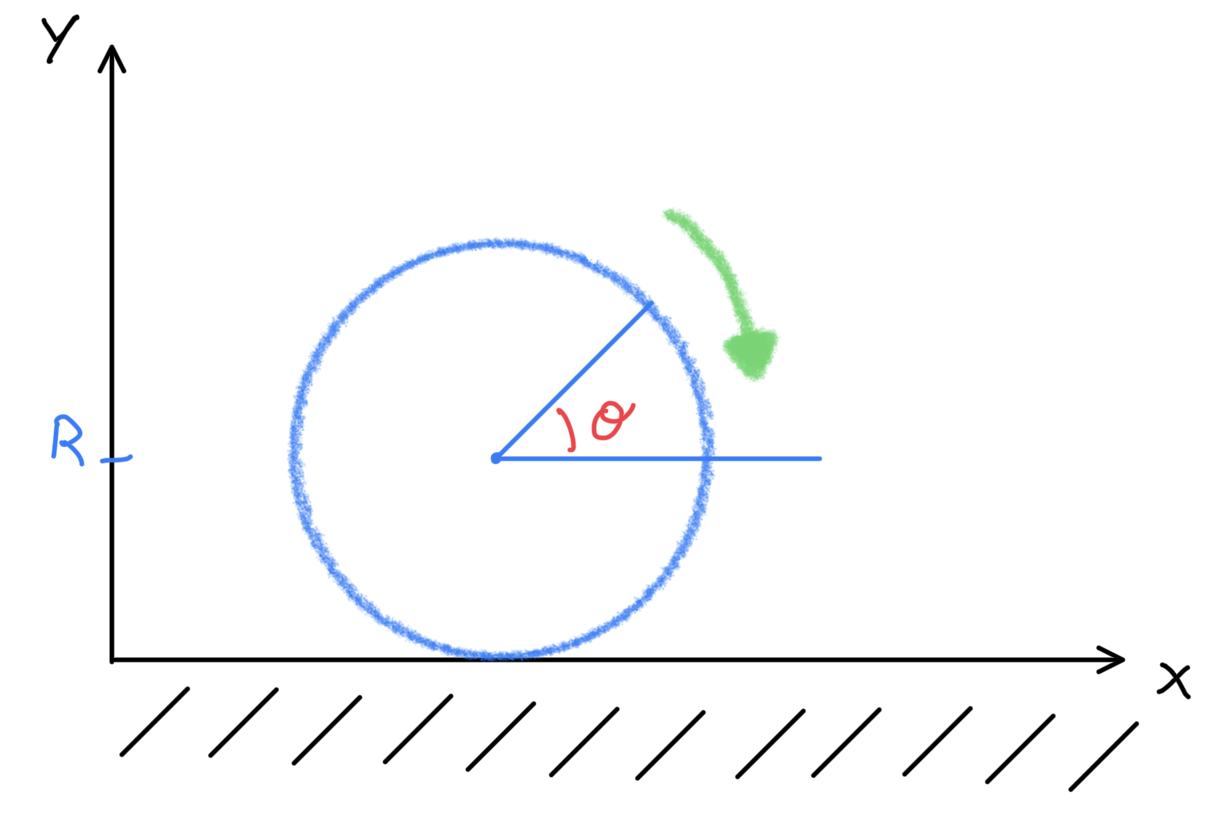
\includegraphics[width=0.48\textwidth]{attrito}
  \end{center}
\end{wrapfigure}
Si consideri un disco che rotola. Per descrivere la sua dinamica \`{e} necessario conoscere la poiszione del centro di massa e dell'angolo di rotazione. La coordinata $y_c = R$ \`{e} costante lungo tutto il moto, ipotizziamo inoltre che il rotolamento avvenga senza strisciare. Di conseguenza la velocit\`{a} lungo l'asse delle ascisse si lega alla velocit\`{a} di rotazione nel seguente modo
\begin{equation*}
	\dot{x}_c = - R\dot{\theta} \Rightarrow \dot{x}_c  = - R \frac{d\theta}{dt}
\end{equation*}
quindi ci si riconduce ad un vincolo olonomo dato da 
\begin{equation*}
	x + R \theta = C
\end{equation*}
\subsubsection{Esempio}
\begin{wrapfigure}{r}{0.5\textwidth}
  \begin{center}
    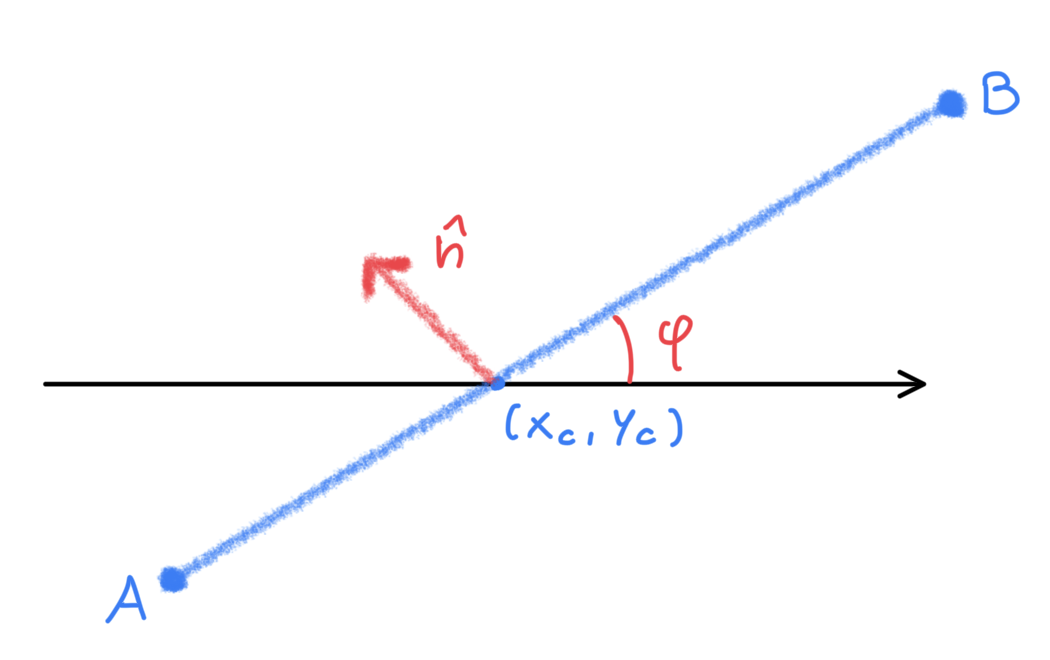
\includegraphics[width=0.48\textwidth]{asta}
  \end{center}
\end{wrapfigure}
Si consideri un problema a 3 g.d.l. dato dalle coordinate $(x_c,y_c,\varphi)$ la veloct\`{a} dell'asta deve avere direzione sempre lungo il segmento $\overline{AB}$. Tale condizione  \`{e} esprimibile andando a considerare un versore $\hat{\bm{n}} = (sin\varphi, - cos\varphi)$ ortogonale al segmento $\overline{AB}$ tale che 
\begin{equation*}
	<\bm{\dot{x}},\hat{\bm{n}}> = 
x_c \sin \varphi-\dot{y}_c \cos \varphi=0 
\end{equation*}
Possiamo domandarci se sia possibile definire una funzione che dipende solo dalle coordinate il cui differenziale \`{e} dato da 
\begin{equation*}
	df(x_{c},y_{c},\varphi) = sin\varphi dx_c - cos\varphi dy_c + 0 d\varphi
\end{equation*}
la risposta \`{e} negativa in quanto il rotore del campo \`{e} nullo
\begin{equation*}
\nabla \times 
\left(\begin{array}{c}
\sin \varphi \\
-\cos \varphi \\
0
\end{array}\right) = 0
\end{equation*} 
di conseguenza non \`{e} una forma chiusa e quindi il vincolo risulta essere Anolonomo.

\section{Vincoli dipendenti dal tempo e velocit\`{a} virtuali}
Ipotizziamo dia vere un vincolo dipendente esplicitamente dal tempo come per esempio un anello il cui raggio cambia nel tempo. Chiedere che la reazione vincolare compia lavoro nullo \`{e} sbagliato dato che questa cambia nel tempo; di conseguenza la condizione di vincolo liscio per scrivere le equazione di E-L dall'energia deve essere modificata e per farlo introduciamo le \textbf{velocit\`{a} virtuali}.
\begin{definition}
	Si definisce velocit\`{a} virtuale la grandezza 
	\begin{equation}
		\bm{v}_{virt} = \frac{d \bm{x}}{dt}-\frac{\partial \bm{x}}{\partial t}
	\end{equation}
\end{definition}
Ridefiniamo la condizione di vincolo liscio chiedendo che la potenza dei vincoli $\bm{\phi}$ sia nulla lungo le velocit\`{a} virtuali.
\begin{equation}
	\pi^{totale} = \bm{F}^{totale} \cdot \bm{v}_{virtuali} = \bm{F}^{attive} \cdot \bm{v}_{virtuali}
\end{equation}
Dimostriamo che le equazioni di E-L per una Lagrangiana $\mathcal{L}(q,\dot{q},t)$ esplicitamente dipendente dal tempo coincidono con quelle di una Lagrangiana indipendente. Per farlo utilizziamo il procedimento usato nella sezione precedente
\begin{equation}
	\pi^{attive} = \bm{F}^{attive} \cdot \bm{v}_{virtuali} 
\end{equation}
per semplicit\`{a} consideriamo un grado di libert\`{a} e dei punti del l'equazione 3.33 \`{e} equivalente a scrivere 
\begin{equation}
\left(\ddot{x} \frac{\partial x}{\partial q} \dot{q}+\ddot{z} \frac{\partial z}{\partial q} \dot{q}\right)=\left(f_x \cdot \frac{\partial x}{\partial q} \dot{q}+f_z \cdot \frac{\partial z}{\partial q} \dot{q}\right)
\end{equation}
ed ipotizziamo anche che le forze arrive siano conservative, ovvero
\begin{equation}
\bm{F}^{attive}=\left(-\frac{\partial U}{\partial x},-\frac{\partial U}{\partial z}\right)
\end{equation}
e quindi la 3.34 assume la forma 
\begin{equation}
\left(\ddot{x} \frac{\partial x}{\partial q}+\ddot{z} \frac{\partial z}{\partial q}\right)=-\left[\frac{\partial U}{\partial x} \cdot \frac{\partial x}{\partial q}+\frac{\partial U}{\partial z} \frac{\partial z}{\partial q}\right] = - \frac{\partial U}{\partial q}
\end{equation}
Prima di riscrivere i termini di sinistra introduciamo due lemmi
\begin{lemma}
	\begin{equation}
		\frac{\partial x}{\partial q} = \frac{\partial \dot{x}}{\partial \dot{q}}
	\end{equation}
\end{lemma}
\begin{proof}
\begin{equation}
	\frac{\partial \dot{x}}{\partial \dot{q}} = \frac{\partial}{\partial \dot{q}}\left(\frac{d}{d t} x(q, t)\right)=\frac{\partial}{\partial \dot{q}}\left(\frac{\partial x}{\partial q} \dot{q}+\frac{\partial x}{\partial t}\right)=\frac{\partial x}{\partial q}
\end{equation}
	
\end{proof}
\begin{lemma}
	\begin{equation}
		 \frac{d}{d t}\left[\frac{\partial x}{\partial q}\right]=\frac{\partial \dot{x}}{\partial q}
	\end{equation}
\end{lemma}
\begin{proof}
	\begin{equation}
\frac{d}{d t}\left[\frac{\partial x}{\partial q}\right]=\frac{\partial}{\partial q}\left(\frac{\partial x}{\partial q} \dot{q}\right)+\frac{\partial}{\partial q} \frac{\partial x}{\partial t}=\frac{\partial}{\partial q} \underbrace{\left[\frac{\partial x}{\partial q} \dot{q}+\frac{\partial x}{\partial t}\right]}_{\dot{x}} = \frac{\partial \dot{x}}{\partial t}
\end{equation}
\end{proof}
\noindent Uno degli addendi di sinistra pu\`{o} essere espresso come 
\begin{equation}
\ddot{x} \frac{\partial x}{\partial q}=\left(\frac{d}{d t}(\dot{x})\right) \frac{\partial x}{\partial q}=\frac{d}{d t}\left(\dot{x} \frac{\partial x}{\partial q}\right)-\dot{x} \frac{d}{d t}\left(\frac{\partial x}{\partial q}\right)
\end{equation}
e applicando i lemmi precedenti la parte di sinistra dell'equazione 3.36 diventa 
\begin{equation}
\begin{aligned}
&  \frac{d}{d t}\left(\dot{x} \frac{\partial \dot{x}}{\partial \dot{q}}+\dot{z} \frac{\partial \dot{z}}{\partial \dot{q}}\right)-m\left[\dot{x} \frac{\partial \dot{x}}{\partial q}+\dot{z} \frac{\partial \dot{z}}{\partial q}\right]= \\[0.2in]
& =\frac{d}{d t} \frac{\partial}{\partial \dot{q}}\left[\frac{1}{2}\left(\dot{x}^2+\dot{z}^2\right)\right]-\frac{\partial}{\partial q} \frac{1}{2} \left(\dot{x}^2+\dot{z}^2\right)
\end{aligned}
\end{equation}
e dunque le equazioni E-L sono date da 
\begin{equation}
\frac{d}{d t} \frac{\partial}{\partial \dot{q}} K-\frac{\partial K}{\partial q}=-\frac{\partial U}{\partial q} \iff 
\frac{d}{d t}\left[\frac{\partial}{\partial \dot{q}} \mathcal{L}(q, \dot{q})\right]=\frac{\partial}{\partial q} \mathcal{L}(q, \dot{q})
\end{equation}

\begin{remark}
Nelle equazioni precedenti si \`{e} assunto che la massa del punto materiale fosse m = 1.	
\end{remark}

\section{Equazioni di E-L dalle equazioni di Newton}
Consideriamo N particelle nello spazio, definiamo la configurazione complessiva del sistema in unico vettore posizione $\bm{x}= \bm{x}(x_1,...,x_{3N})$. Ipotizziamo di parametrizzare le $x_j$ rispetto alle coordinate generalizzate $(q_1,..,q_d)$.
\begin{equation}
\left\{\begin{array}{l}
x_1 = \varphi\left(q_1, \ldots  q_d, t\right) \\
x_2 = \varphi\left(q_1, \ldots, q_d, t\right) \\
\quad \vdots \\
x_{3 N} = \varphi\left(q_1, \ldots, q_d, t\right)
\end{array}\right.
\end{equation}
le velocit\`{a} generalizzate per una singola componente assumono la forma 
\begin{equation}
	\frac{dx_i}{dt} = \sum_{j=1}^d \frac{\partial x_i}{\partial q_j}\dot{q}_j + \frac{\partial x_i}{\partial t}
\end{equation}
Costruiamo le velocit\`{a} virtuali definendo le singole componenti del vettore $\bm{v}_{virtuali}$ come
\begin{equation}
v_{i}=\frac{d x_i}{d t}-\frac{\partial x_i}{\partial t}=\sum_{j=1}^d \frac{\partial x_i}{\partial q_j} \dot{q}_j
\end{equation}
consideriamo N  vincoli olonomi e lisci, e definiamo un unico vettore $\bm{\phi}$ tale che la potenza dei vincoli in ogni punto lungo le velocit\`{a} virtuali \`{e} nulla. Si definisce in questo modo il principio di D'Alambert 
\begin{equation}
	\sum_{k=1}^{N} \bm{\phi}_{k} \cdot \bm{v}_{k} = 0 
\end{equation}
La potenza totale del sistema \`{e} data da 
\begin{equation}
	\pi^{totale} = \sum_{k=1}^{N}m_k \bm{a}_k \cdot \bm{v}_{k} = \sum_{k=1}^{N} \bm{F}_{k}^{attive} \cdot \bm{v}_{k} + \underbrace{ \sum_{k=1}^{N} \bm{\phi}_{k} \cdot \bm{v}_k }_{=0}
\end{equation}
Come fatto per un solo grado di libert\`{a} assumiamo che $\bm{F}^{attiva}$ sia una forza conservativa e dunque 
\begin{equation}
\bm{F}^{attive}	= - \nabla U(x_1,..,x_{3n})
\end{equation}
 dunque possiamo riscrivere il termine di destra rimanente in 3.48 come 
 \begin{equation}
 	\sum_{k=1}^{N} \bm{F}_{k}^{attive} \cdot \bm{v}_{k} = 
-\sum_{j=1}^d \sum_{i=1}^{3 N} \frac{\partial U}{\partial x_i} \frac{\partial x_i}{\partial q_j} \dot{q}_j = 
-\sum_{j=1}^d \frac{\partial U}{\partial q_j} \dot{q}_j
\end{equation}
mentre il termine di destra diventa 
\begin{equation}
\sum_{j=1}^d \Big [\sum_{i=1}^{3 N} m_i \underbrace{\ddot{x}_i \frac{\partial x_i}{\partial q_j}}_{A}\Big ]\dot{q}_j
\end{equation}
il termine A pu\`{o} essere riscritto come
\begin{equation}
\ddot{x}_i \frac{\partial x_i}{\partial q_j}=\frac{d}{d t} \dot{x}_j \frac{\partial x_i}{\partial q_j}=\frac{d}{d t}\left(\dot{x}_i \frac{\partial x_i}{\partial q_j}\right)-\dot{x}_i \frac{d}{d t} \frac{\partial x_i}{\partial q_j}
\end{equation}
ottenuto dai due lemmi precedenti. Sostituendo in 3.51 otteniamo
\begin{equation}
\frac{d}{d t}\left[\sum_{i=1}^{3 N} m_i \dot{x}_i \frac{\partial \dot{x}_i}{\partial q_j}\right]-\sum_{i=1}^{3 N} m_i \dot{x}_i \frac{\partial\dot{x}_i}{\partial q_j} 
\end{equation}
che rispettivamente rappresentano
\begin{equation}
\frac{\partial}{\partial \dot{q}_j}\left(\frac{1}{2} \sum_{i=1}^{3 N} m_i \dot{x}_i^2\right) \quad \text{e} \quad 
\frac{\partial K}{\partial q_j} 
\end{equation}
in conclusione 
\begin{equation}
\sum_{j=1}^d\left(\frac{d}{d t} \frac{\partial K}{\partial \dot{q}_j}-\frac{\partial K}{\partial q_j}\right) \dot{q}_j=-\sum_{j=1}^d \frac{\partial U}{\partial q_j} \dot{q}_j \quad \forall \dot{q}_j
\end{equation}
e tale risultato equivale ad un sistema di d equazioni di Eulero Lagrange 
\begin{equation}
\left\{\begin{aligned}
\frac{d}{d t} \frac{\partial \mathcal{L}}{\partial \dot{q}_j} & =\frac{\partial \mathcal{L}}{\partial q_j} \\
\forall j & =1, \ldots, d
\end{aligned}\right.
\end{equation}

\section{Lagrangiana ridotta}

\begin{definition}
	Si consideri una Lagrangiana $\mathcal{L}(q_1,..,q_d,\dot{q}_1,..,\dot{q}_d,t)$ che non dipende esplicitamente dalla coordinate $q_j$, allora si dice che $q_j$ \`{e} una \textbf{variabile ciclica}.
\end{definition}
\noindent Dunque se $q_j$ \`{e} una variabile ciclica si ha che $\frac{\partial \mathcal{L}}{\partial q_j} = 0$ di conseguenza dalle equazioni di E-L si ha che $\frac{d}{dt} \frac{\partial \mathcal{L}}{\partial \dot{q}_j} = 0$ e quindi $\frac{\partial \mathcal{L}}{\partial \dot{q}_j}$ \`{e} una costante del moto, ed \`{e} esprimibile come
\begin{equation}
	\frac{\partial \mathcal{L}}{\partial \dot{q}_j} = C(q_1,..,q_{d-1},\dot{q}_1,..,\dot{q}_{d-1})
\end{equation}
dalle equazioni di E-L possiamo esplicitare $\dot{q}_j$ rispetto le altre coordinate e velocit\`{a} generalizzate 
\begin{equation}
	\dot{q}_j = f(q_1,..,q_{d-1},\dot{q}_1,..,\dot{q}_{d-1})
\end{equation}
Abbiamo visto che per una Lagrangian indipendente dal tempo, l'energia cinetica \`{e} una costante del moto
\begin{equation}
	E(q_1,..,q_d,\dot{q}_1,..,\dot{q}_d) = K(q_1,..,q_d,\dot{q}_1,..,\dot{q}_d) + U(q_1,..,q_d)
\end{equation}
sostituiamo rispetto $\dot{q}_j$ all'interno dell'equazione dell'energia. In questo modo i termini dell'energia coincidono con quella di una Lagrangiana con energia cinetica $\tilde{K}$ e un potenziale efficace $U_{eff}$.
\begin{equation}
	\mathcal{L} = \tilde{K} + U_{eff}
\end{equation}
tale funzione prende il nome di \textbf{Lagrangiana ridotta} poich\`{e} i gradi di libert\`{a} ottenuti sono minori di quelli della Lagrangiana di partenza.

\section{Punti di equilibrio di un sistema per 1 g.d.l.}

Consideriamo inizialmente il caso per un solo grado di libert\`{a}, ed esprimiamo esplicitamente la dipendenza della Lagrangiana rispetto G(q) funzione dell'energia cinetica
\begin{equation}
	\mathcal{L}(q,\dot{q}) = \frac{1}{2}G(q)\dot{q}^2 - U(q)
\end{equation}
i termine delle equazioni di E-L sono 
\begin{equation}
	\frac{d}{d t}\left(\frac{\partial \mathcal{L}}{\partial \dot{q}}\right)=G^{\prime}(q) \dot{q}^2+G(q) \ddot{q}  \quad \text{e} \quad 
	\frac{\partial \mathcal{L}}{\partial q}(q, \dot{q})=\frac{1}{2} \frac{d G}{d q} \dot{q}^2-\frac{d U}{d q}
\end{equation}
e quindi 
\begin{equation}
\begin{aligned}
G^{\prime} \dot{q}^2+G(q) \ddot{q} & =\frac{1}{2} G^{\prime}(q) \dot{q}^2-U^{\prime} \\
G(q) \ddot{q} & =-\frac{1}{2} G^{\prime}(q) \dot{q}^2-U^{\prime} \\
\ddot{q} & =-\frac{1}{2} \frac{G^{\prime}(q)}{G(q)} \dot{q}^2-\frac{U^{\prime}}{ G\left (q \right)}
\end{aligned}
\end{equation}
l'ultimo termine prende il nome di \textbf{forma normale dell'equazioni di Eulero Lagrange}. Riscrivendo l'equazione di E-L in forma normale otteniamo una EDO del secondo grado che pu\`{o} essere riscritta come sistema di EDO del primo ordine 
\begin{equation}
\left\{\begin{array}{l}
y=\dot{q} \\
\dot{y}=-\frac{1}{2} \frac{G^{\prime}(q)}{G(q)} y^2-\frac{U^{\prime}(q)}{G(q)}
\end{array}\right.
\end{equation}
Dalla teoria dei sistemi dinamici al capitolo due sappiamo che le soluzioni sono stazionarie se sono del tipo $(\bar{q},0)$ e rispetto al nostro sistema dobbiamo dunque imporre che $U^{\prime} (\bar{q}) = 0$. Dunque per trovare le soluzioni stazionarie del problema vincolato dobbiamo trovare i punti compatibili con vincolo tali per cui la derivata prima del potenziale del sistema si annulla.
\newline

\noindent Una domanda che possiamo porci \`{e}: \textbf{come determiniamo la stabilit\`{a} dei punti ?}
\subsection{Stabilit\`{a} dei punti di equilibrio per 1 g.d.l.}
 Applichiamo il secondo teorema di Lyapunov, che ci dice che per un sistema dinamico l'energia \`{e} una buona funzione di Lyapunov essendo una costante del moto rispetto alle velocit\`{a} e coordinate generalizzate.
 
 \noindent Per determinare la stabilit\`{a} del punto stazionario $(\bar{q},0)$, studiamo il segno della matrice Hessiana dell'energia del sistema.
 \begin{equation}
H(\bar{q}, 0)=\left[\begin{array}{cc}
U^{\prime \prime}(\bar{q}) & 0 \\
0 & G(\bar{q})
\end{array}\right]
\end{equation}
Affinch\`{e} $(\bar{q},0)$ sia un punto di minimo per l'energia \`{e} necessario che $U^{\prime\prime}(\bar{q}) > 0 $ in modo che la matrice Hessiana sia definita positiva. Per i teoremi di Lyapunov tale punto risulta essere di equilibrio stabile.

\subsection{Linearizzazione del sistema attorno a un punto di equilibrio stabile per 1 g.d.l.}

Dato un punto di equilibrio stabile $(\bar{q},0)$ per il sistema definito in 3.64, ipotizziamo si perturbare la soluzione do una quantit\`{a} $\varepsilon$ lungo una direzione $\bm{h}$
\begin{equation}
\left\{\begin{array}{l}
q(t)=\bar{q}+\varepsilon u(t) \\
y(t)=0+\varepsilon v(t)
\end{array}\right.
\end{equation}
Possiamo procedere in due modi per determinare come il sistema cambi rispetto ad una variazione infinitesima
\begin{itemize}
	\item \textbf{$\bm{I}^{\circ}$ metodo:} Sostituiamo la soluzione perturbata all'interno delle equazioni del sistema in 3.64
	\begin{equation}
\left\{\begin{array} { l } 
{ \dot { q } = \varepsilon \dot { u } } \\
{ \dot { \varphi } = \varepsilon \dot { v } }
\end{array} \rightarrow \left\{\begin{array}{l}
\varepsilon \dot{u}=\varepsilon v \\
\varepsilon \dot{v}=-\frac{1}{2} \frac{G^{\prime}(\bar{q}+\varepsilon u(t))}{G(\bar{q}+\varepsilon u(t))} \varepsilon^2 v^2-\frac{U^{\prime}(\bar{q}+\varepsilon u(t))}{G(\bar{q}+\varepsilon u(t))}
\end{array}\right.\right.
\end{equation}
che possiamo riscrivere come 
\begin{equation}
\varepsilon G(\bar{q}+\varepsilon u(t)) \dot{v}=-\frac{1}{2} G^{\prime}(\bar{q}+\varepsilon u(t)) \varepsilon^2 v^2-U^{\prime}(\bar{q}+\varepsilon u(t))
\end{equation}
espandiamo l'equazione 3.68 con Taylor al secondo ordine in un'intorno del punto di equilibrio
\begin{equation}
\left\{\begin{array}{l}
\dot{u}=v \\
G(\bar{q}) \dot{v}=-U^{\prime \prime}(\bar{q}) u
\end{array}\right.
\end{equation}
ottenendo l'equazione differenziali al secondo ordine i u di un'oscillatore armonico
\begin{equation}
\ddot{u}=-\left(\frac{U^{\prime \prime}(\bar{q})}{G(\bar{q})}\right)u
\end{equation}
\item \textbf{$\bm{II}^{\circ}$ metodo:} Sostituiamo la soluzione definita in 3.66 nella Lagrangiana e si sviluppa al secondo ordine usando Taylor in un intorno della soluzione 
\begin{equation}
\mathcal{L}(q,\dot{q})=\frac{1}{2} G(\bar{q}+\varepsilon u) \varepsilon^2 \dot{u}^2-U(\bar{q}+\varepsilon u)
\end{equation}
in questo modo si ottiene la Lagrangiana linearizzata 
\begin{equation}
\begin{aligned}
&\tilde{\mathcal{L}}(u, \dot{u})\approx \frac{1}{2} G(\bar{q}) \varepsilon^2 \dot{u}^2-U(\bar{q})+U^{\prime}(\bar{q}) \varepsilon u+\frac{U^{\prime \prime}}{2}(\bar{q}) \varepsilon^2 u^2 =& \\[0.15in]
& = \left[\frac{1}{2} G(\bar{q}) \dot{u}^2-\frac{U^{\prime \prime}}{2}(\bar{q}) u^2\right] \varepsilon^2 - U(\bar{q})
\end{aligned}
\end{equation}
Le componenti dell'equazione di E-L associate alla Lagrangiana linearizzata saranno date da 
\begin{equation}
\frac{d}{d t}\left[\frac{\partial \tilde{\mathcal{L}}}{\partial \dot{u}}(u, \dot{u})\right]  =\varepsilon^2 G(\bar{q}) \ddot{u} \quad \text{e} \quad
{\left[\frac{\partial \tilde{\mathcal{L}}}{\partial u}(u, \dot{u})\right] }  =-\varepsilon^2 U^{\prime \prime}(\bar{q}) u
\end{equation}
e l'equazione
\begin{equation}
	\ddot{u} = -\frac{U^{\prime \prime}(\bar{q})}{G(\bar{q})}u
\end{equation}
che coincide con l'equazione differenziale di un oscillatore armonico.
\end{itemize}
Prende il nome di \textbf{piccola oscillazione} il termine 
\begin{equation}
	\omega^2 =  \frac{U^{\prime \prime}(\bar{q})}{G(\bar{q})}
\end{equation} 
\section{Punti di equilibrio di un sistema per N g.d.l.}
Nella sezione precedente abbiamo visto che per sviluppare con Taylor in un intorno di un punto di equilibrio stabile ci restituisce l'equazione di un oscillatore armonico. Nel caso in pi\`{u} gradi di libert\`{a} iniziamo con lo studiare la struttura della matrice dell'energia cinetica.
\subsection{Matrice dell'energia cinetica}
Prendiamo un unico vettore per N punti materiali nello spazio $\bm{x} = (x_1,...,x_{3N})$ con le rispettive masse $\bm{m} = (m_1,...,m_{3N})$, e ipotizziamo che la parametrizzazione delle coordinate di posizione sia data da quelle coordinate, ma anche dal tempo $x_i = x_i(q_1,...,q_d,t)$, allora l'energia cinetica del sistema \`{e} data da 
\begin{equation}
	K = \frac{1}{2}\sum_{i=1}^{3N}m_i \dot{x}_{i}^2
\end{equation}
dove il termine della velocit\`{a} rispetto alle coordinate pu\`{o} essere definito in relazione delle coordinate generalizzate nel seguente modo
\begin{equation}
	\dot{x}_{i} = \sum_{j=1}^{d} \frac{\partial x_i}{\partial q_j}\dot{q}_j + \frac{\partial x_i}{\partial t}
\end{equation}
il termine quadratico nell'equazione dell'energia cinetica assume la forma 
\begin{equation}
\dot{x}_i^2=\sum_{r, s=1}^d \frac{\partial x_i}{\partial q_r} \dot{q}_r \frac{\partial x_i}{\partial q_s} \dot{q}_s+\underbrace{\left(\frac{\partial x_i}{\partial t}\right)^2+ 2 \frac{\partial x_i}{\partial t} \sum_{r=1}^d \frac{\partial x_j}{\partial q_r} \dot{q}_r}_{= B}
\end{equation}
di conseguenza la forma dell'energia cinetica rispetto alle coordinate generalizzate \`e data da 
\begin{equation}
K=\frac{1}{2} \sum_{i=1}^{3 N} m_i\left[\sum_{r, s=1}^d \frac{\partial x_i}{\partial q_r} \dot{q}_r \frac{\partial x_i}{\partial q_s} \dot{q}_s\right]+\frac{1}{2} \sum_{i=1}^{3 N} m_i B
\end{equation}
dove il termine B compare solo se le coordinate spaziale hanno una dipendenza esplicita dal tempo. Nel caso in cui questo non sia vero si ha che l'equazione 3.79 \`{e} data da 
\begin{equation}
	\begin{aligned}
	K(q,\dot{q}) = \frac{1}{2} \sum_{i=1}^{3 N} m_i\left[\sum_{r, s=1}^d \frac{\partial x_i}{\partial q_r} \dot{q}_r \frac{\partial x_i}{\partial q_s} \dot{q}_s\right] = \\[0.1in] 
	=\frac{1}{2} \sum_{r,s =1}^{d} \left [ \sum_{i=1}^{3N} m_i \frac{\partial x_i}{\partial q_r} \frac{\partial x_i}{\partial q_s} \right ]\dot{q}_r\dot{q}_s 
	\end{aligned}
\end{equation}
che possiamo riscrivere in forma vettoriale come 
\begin{equation}
	K(q,\dot{q}) = \frac{1}{2} \left [ \dot{q}_1,...,\dot{q}_d\right] \cdot G(q_1,..,q_d) \cdot \left [  \begin{array}{c}
		\dot{q}_1 \\
		\vdots \\
		\dot{q}_d \\
	\end{array}\right] 
\end{equation}
dove $G(q_1,..,q_d)$ \`{e} prende il nome di \textbf{matrice dell'energia cinetica}. Tale matrice \`{e} una forma bilineare, simmetrica e definita positiva, ovvero per ogni scelta del vettore $\bm{\dot{q}} \neq 0$ si ha che $\sum_{r,s=1}^{3N}G_{r,s} \dot{q}_r \dot{q}_s > 0$.

\subsection{Linearizzazione del sistema attorno ad un punto di equilibrio stabile per N g.d.l.} 

Rispetto all'espressione 3.80 possiamo scrivere la Lagrangiana del sistema come 
\begin{equation}
	\mathcal{L}(q_1,..,q_d,\dot{q}_1,..,\dot{q}_d) = \frac{1}{2} \sum_{r,s=1}^{3N}G_{rs}(q_1,..,q_d)\dot{q}_r\dot{q}_s - U(q_1,..,q_d)
\end{equation}
dato $\bm{q}^{*}$ tale per cui $\nabla U(\bm{q}^{*}) = 0$ che equivale a imporre che $\frac{\partial U}{\partial q_j} = 0 \quad \forall \; j = 1,..,d$ e $H_{U}(\bm{q}^{*})$ matrice Hessiana dell'energia potenziale definita positiva  si ha che $(\bm{q}^{*},0)$ \`{e} un punto di equilibrio stabile secondo Lyapunov. Come fatto nel caso ad 1 g.d.l. procediamo a perturba la soluzione di un fattore $\varepsilon$ lungo una certa direzione \textbf{u} e studiare le propriet\`{a} del sistema perturbato.
Rispettivamente avremo 
\begin{equation}
\bm{q}(t)=\bm{q}{*}+\varepsilon \bm{u}(t) \quad \bm{\dot{q}}=\varepsilon \dot{\bm{u}}, \quad \ddot{\bm{q}}=\varepsilon \ddot{\bm{u}}
\end{equation}
definiamo il sistema di equazioni di E-L come 
\begin{equation}
\left \{ \begin{array}{l}
\sum_{\beta = 1}^d G_{\gamma \beta} \ddot{q}_\beta=\sum_{\alpha, \beta=1}^d \Gamma_{\alpha \beta \gamma} \dot{q}_\alpha \dot{q}_\beta-\frac{\partial U}{\partial q_\gamma} \\ 
\forall \; \gamma =1,...,d
\end{array} \right .
\end{equation}
per lo studio delle equazioni possiamo procedere in due modi differenti che riconducono al medesimo risultato
\begin{itemize}
	\item \textbf{$\bm{I}^{\circ}$ metodo:} Si procede a sostituire la soluzione perturbata all'interno delle equazioni di E-L e sviluppare con Taylor fino al primo ordine in un suo intorno.
	\begin{equation}
\sum_{\beta = 1}^d G_{\gamma \beta}\left(\bm{q}^*+\varepsilon \bm{u}\right) \varepsilon \ddot{u}_\beta=\sum_{\alpha, \beta}^d \Gamma_{\alpha, \beta, \gamma}\left(\bm{q}^*+\varepsilon \bm{u}\right) \varepsilon^2 \dot{u}_\alpha \dot{u}_\beta-\frac{\partial U}{\partial q_\gamma}\left(\bm{q}^*+\varepsilon \bm{u}\right)
\end{equation}
procedendo con Taylor fissando $\gamma$ si ottiene 
\begin{equation}
\begin{aligned}
& \left[\sum_{\beta=1} G_{\gamma \beta}\left(\boldsymbol{q}^*\right) \ddot{u}_\beta\right] \varepsilon=-\left[\frac{\partial U\left(\boldsymbol{q}^*\right)}{\partial q_\gamma}+\frac{\partial^2 U\left(\boldsymbol{q}^*\right)}{\partial q_\gamma \partial q_1} \varepsilon u_1+\ldots+\frac{\partial^2 U\left(\boldsymbol{q}^*\right)}{\partial q_\gamma \partial q_d} \varepsilon u_d\right]\\[0.2in]
& {\left[\sum_{\beta = 1} G_{\gamma \beta}\left(\bm{q}^*\right) \ddot{u}_\beta\right] \varepsilon=-\frac{\partial U\left(\bm{q}^*\right)}{\partial q_\gamma}-\varepsilon \sum_{\alpha=1}^d \frac{\partial^2 U\left(\bm{q}^*\right) }{\partial q_\gamma \partial q_\alpha}}u_\alpha = \\[0.2in]
&{\left[\sum_{\beta = 1} G_{\gamma \beta}\left(\bm{q}^*\right) \ddot{u}_\beta\right] =-\sum_{\alpha=1}^d \frac{\partial^2 U\left(\bm{q}^*\right) }{\partial q_\gamma \partial q_\alpha}}u_\alpha
\end{aligned}
\end{equation}
dove i termini di destra e sinistra coincidono rispettivamente con 
\begin{equation}
\left[\sum_{\beta = 1} G_{\gamma \beta}\left(\bm{q}^*\right) \ddot{u}_\beta\right] = \left [ G_{0} \ddot{\bm{u}} \right ]_{\gamma} \quad \quad \sum_{\alpha=1}^d \frac{\partial^2 U\left(\boldsymbol{q}^*\right)}{\partial q_\gamma \partial q_\alpha} u_\alpha = \left [ H_0 \bm{u} \right ]_{\gamma}
\end{equation}
dunque le equazione del moto linearizzate coincidono con il sistema
\begin{equation}
	\boxed{G_0 \bm{\ddot{u}} = -H_0 \bm{u}}
\end{equation}
\item \textbf{$\bm{II}^{\circ}$ metodo:} Si sostituisce la soluzione perturbata all'interno della Lagrangiana del sistema e si procede ad espandere al primo ordine con Taylor in un suo intorno.
\begin{equation}
\begin{aligned}
&\mathcal{L}(\bm{q}^{*}+\varepsilon\bm{u},\varepsilon\bm{\dot{u}}) \approx \frac{1}{2} \sum_{r,s=1}^{3N} G_{rs}(\bm{q}^{*}+\varepsilon \bm{u})\varepsilon^2 \dot{u}_r \dot{u}_s - U(\bm{q}^{*}+ \varepsilon \bm{u}) = \\
& = \frac{1}{2} \sum_{r,s=1}^{3N} G_{rs}(\bm{q}^{*})\varepsilon^2 \dot{u}_r \dot{u}_s - U(\bm{q}^{*}) - \frac{1}{2} \varepsilon^2 \sum_{r,s = 1}H_{rs}(\bm{q}^{*})u_r u_s = & \\
& = \frac{1}{2} \left [\sum_{r,s=1}^{3N} G_{rs}(\bm{q}^{*}) \dot{u}_r \dot{u}_s  - \varepsilon^2 \sum_{r,s = 1}H_{rs}(\bm{q}^{*}) u_r u_s \right ]\varepsilon^2- U(\bm{q}^{*})
\end{aligned}
\end{equation}
calcolando le equazioni di E-L rispetto alla Lagrangiana linearizzata otteniamo gli stessi elementi in 3.87  e di conseguenza si ottiene l'equazione 3.88.
\end{itemize}

\subsection{Frequenze proprie e modi normali di oscillazione}

Data una Lagrangiana linearizzata in un intorno di un punto di equilibrio stabile dall'equazione 3.88 otteniamo un sistema di oscillatori armonici
\begin{equation}
	\left \{ \begin{array}{l}
	\ddot{u}_{\gamma} = - \frac{H_0^{s \gamma }}{G_0^{s \gamma }}u_{\gamma} \\
	\forall \; \gamma = 1, \cdots, d
	\end{array} \right.
\end{equation}
cerchiamo una soluzione del sistema della forma 
\begin{equation}
	\bm{u}(t) = \bm{w}\; cos(\omega t + \phi) 
\end{equation}
ovvero tutti i gradi di libert\`{a} oscillano con la stessa pulsazione ed ampiezze $\bm{w}$ diverse ed indipendenti dal tempo. Procediamo a sostituire il guess 3.91 all'interno dell'equazione 3.88 ottenendo la relazione 
\begin{equation}
	(\omega^2 G_0 - H_0)\bm{u} = 0 \iff (\omega^2 G_0 - H_0)cos(\omega t + \phi) \bm{w} = 0 
\end{equation}
affinch\`{e} tale relazione sia soddisfatta per ogni tempo t \`{e} necessario che $\bm{w} \in Ker[\omega^2 G_0 -H_0]$.
\newline
La grandezza $\omega$ prende il nome di \textbf{pulsazione propria}, mentre l'ampiezza data dal vettore $\bm{w}$ viene definita \textbf{modi normali di oscillazione}. La soluzione generale del sistema \`{e} data dalla sovrapposizione lineare di ciascun modo di oscillazione 
\begin{equation}
	\bm{u}(t) =  \bm{q}^{*} + \sum_{i=1}^{k}   \bm{w}_{i} \; sin(\omega_i t + \phi_i)  + \sum_{j=1}^{k}  \bm{w}_{j} \; cos(\omega_j t + \phi_j)
\end{equation}
rispettivamente le pulsazioni proprie $\omega$ e i modi normali $\bm{w}$ sono gli autovalori e autovettori della matrice M.
\subsection{Stabilit\`{a} delle soluzioni stazionare per un sistema Lagrangiano}

Le equazioni del moto rispetto alle coordinate generalizzate per una Lagrangiana linearizzata in un intorno di un punto di equilibrio sono
\begin{equation}
\left\{\begin{array}{l}
	\dot{\bm{u}}=\bm{y} \\
	\dot{\bm{y}}=-G_0^{-1} H_0 \bm{u}
\end{array}\right.
\end{equation}
che possiamo esprimere in forma matriciale come 
\begin{equation}
\left[\begin{array}{l}
\dot{u} \\
\vdots \\
\dot{y}
\end{array}\right]=\left[\begin{array}{c|c}
0 & I \\
\hline -G_0^{-1} H_0 & 0
\end{array}\right]
\left[\begin{array}{c}
u\\
\vdots \\
y
\end{array}\right] = M
\left[\begin{array}{c}
u\\
\vdots \\
y
\end{array}\right]
\end{equation}
il polinomio caratteristico associato alla matrice M \`{e} dato da $P(\omega) = det (\omega I -M) = 0$ per calcolarlo riscriviamo la matrice $\omega I - M$ come 
\begin{equation}
\left[\begin{array}{c|c}
I & 0 \\
\hline -\frac{1}{\omega}G_0^{-1} H_0 & I
\end{array}\right]\left[\begin{array}{c|c}
\omega I & -I \\
\hline G_0^{-1} H_0 & \omega I
\end{array}\right]=\left[\begin{array}{c|c}
\omega I & -I \\
\hline 0 & \frac{1}{\omega} G_0^{-1} H_0+\omega I
\end{array}\right]
\end{equation}
applicando il teorema di Binet abbiamo che il polinomio caratteristico \`{e} dato da 
\begin{equation}
\begin{aligned}
P(\omega) & =\operatorname{det}(\omega I) \operatorname{det}\left(\omega I+\frac{1}{\omega} G_0^{-1} H_0\right)= \\
& =\operatorname{det}\left(\omega^2 I+G_0^{-1} H_0\right)=\operatorname{det}\left(-G_0^{-1}\left(-\omega^2 G_0-H_0\right)\right) \\
& =\operatorname{det}\left(-G_0^{-1}\right) \operatorname{det}\left(-\omega^2 G_0-H_0\right)= 0
\end{aligned}
\end{equation}
il fattore di destra ci dice che gli autovalori della matrice M coincido con le pulsazioni proprie del sistema linearizzato, ovvero $\lambda_i = - \omega_i^2$.
Supponiamo che $\exists \; i$ tale che  $\lambda_i <0$ allora avremo che $\omega_i = \pm \sqrt{\lambda_i}$ per il $\bm{I^{\circ}}$ \textbf{teorema di Lyapunov}, il punto $(\bm{q}^{*},0)$ \`{e} di equilibrio instabile. Se invece tutte le soluzioni di $P(\lambda) = 0$ sono $\lambda_i > 0 $ si ha che gli $\omega_i$ sono numeri immaginari puri il primo teorema di Lyapunov non \`{e} applicabile. Osserviamo che le  $\lambda_i$ soluzioni del polinomio caratteristico $P(\lambda) = det (\lambda G_0 -H_0) =0$ il numero di autovalori positivi $\lambda_i > 0 $ della matrice $\lambda G_0 -H_0$ coincide con il numero di autovalori positivi $\mu_i >0$ della matrice $H_0$ e in egual modo per quelli negativi, di conseguenza in generale si ha che per una Hessiana definita positiva non si pu\`{o} applicare il $I^{\circ}$ teorema di Lyapunov.\newline
Come facciamo a determinare la stabilit\`{a} dei punti/o di equilibrio in questi casi ? per rispondere a tale domanda introduciamo il seguente teorema.

\begin{theorem}[\textbf{Teorema di Lagrange-Dirichlet}]
Dato un sistema olonomo soggetto a forze conservative e con vincoli perfetti (bilaterali) indipendenti dal tempo, se l'energia potenziale ha un minimo relativo proprio quando il sistema assume una certa configurazione di equilibrio, allora in questo punto il sistema è in equilibrio meccanico stabile, nel senso di Lyapunov.
\end{theorem}
\begin{proof}
		Sappiamo dal $\bm{II^{\circ}}$ \textbf{teorema di Lyapunov} che una buona funzione di Lyapunov \`{e} data dall'energia del sistema 
	\begin{equation}
		E = \frac{1}{2}<\bm{{y}},G(\bm{q})\bm{y}> + U(\bm{q})
	\end{equation}
	allora determiniamo il suo punto di minimo
	\begin{equation}
\nabla E=\left(\frac{1}{2} <\bm{y} ,\frac{\partial G}{\partial q} \bm{y}>+\frac{\partial U}{\partial q}, G(q) \bm{y}\right)=(0,0)
\end{equation}
di conseguenza avremo che $\bm{y} = 0 $ e deve esistere $\bm{q}^*$ tale che $\frac{\partial U}{\partial q} = 0$, dunque $(\bm{q}^{*},0)$ \`{e} un punto stazionario per il sistema di equazioni differenziali e di conseguenza punto di equilibrio. Affinch\`{e} tale punto sia di minimo per l'energia dobbiamo verificare il segno della matrice Hessiana 
\begin{equation}
H_E\left(\bm{q}^*, \bm{0}\right)=\left[\begin{array}{c|c}
H_0\left(\bm{q}^*\right) & 0 \\
\hline 0 & G\left(\bm{q}^*\right)
\end{array}\right]=\left[\begin{array}{c|c}
H_0 & 0 \\
\hline 0 & G_0
\end{array}\right]
\end{equation}
poich\`{e} $H_0$ e $G_0$ sono definite positive si ha per il teorema di Binet che $H_E(\bm{q}^*,\bm{0})$ \`{e} definita positiva, di conseguenza $(\bm{q}^*,\bm{0})$ \`{e} un punto di minimo per l'energia e quindi \`{e} un punto di equilibrio stabile.
 
\end{proof}

\begin{theorem}
	Sia $G_0$ una matrice simmetrica e definita positiva, e sia $H_0$ simmetrica allora:
	\begin{enumerate}
		\item $\exists$ una base di $\mathbb{R}^d$ fatta di autovettori di $H_0$ rispetto a $G_0$.
		\item dati due autovalori distinti $\lambda_i \neq \lambda j$ si ha che $<\bm{w}_i,G_0\bm{w}_j> = 0$
		\item Se $H_0$ \`{e} definita positiva allora $\lambda_i > 0 \quad \forall\,i$ 
	\end{enumerate}
\end{theorem}

\subsection{Il principio di minima azione}

Consideriamo un punto $(q,\dot q) \in \Omega \subseteq \mathbb{R}^{2N}$ elemento dello spazio delle fasi, abbiamo che l'evoluzione della posizione del punto q nel tempo
\begin{equation}
	q : [t_0,t_1] \rightarrow \mathbb{R} \quad \text{t.c} \quad  q(t_0) = q_0 \quad \text{e} \quad q(t_1) = q_1
\end{equation}
definisce un cammino nello spazio delle configurazioni. Il numero di cammini che uniscono due punti nello spazio \`{e} infinito, dunque non \`{e} univoco, ci domandiamo quale sia il reale cammino che congiunge le due posizioni. Per rispondere a tale domanda introduzione una grandezza che \`{e} data dal funzionale d'azione.

\begin{equation}
	S: \mathcal{C}_{0,1} \rightarrow \mathbb{R} 	
\end{equation}
\begin{equation*}
	q \mapsto S[q] 
\end{equation*}
definita sullo spazio dei cammini, che \`{e} uno spazio affine modellato su uno spazio vettoriale di dimensione infinita. Dove 
\begin{equation}
	S\left[q(t)\right]=\int_{t_i}^{t_f} \mathcal{L}\left(q(t), \dot{q}(t)\right) d t
\end{equation}
e $\mathcal{L}$ definisce la Lagrangiana del sistema associata. L'azione  ha una propriet\`{a} significativa rispetto ai cammini di un sistema, ovvero il cammino effettivamente percorso dal sistema coincide con il suo estremo inferiore. 
\begin{lemma}
	Sia g(t) una funzione continua e derivabile in $[t_0,t_1]$ tale che $\forall \,h(t)$ continua in $[t_0,t_1]$ se 
	\begin{equation*}
		\int_{t_0}^{t_1}h \cdot g \;dt = 0 \Rightarrow g = 0
	\end{equation*}
	\end{lemma}
	\begin{proof}
	Sia $g(t) \neq 0$ allora esiste $\tau \in [t_0,t_1]$ tale che $g(\tau) > A $ dove $A>0$ per continuit\`{a} della funzione deve esiste un intorno dove g \`{e} al di sopra di A. Consideriamo un cammino h per cui il $g\cdot h > 0 \;\; \forall \;t$, in particolare in un intervallo di misura non nullo. Allora avremo che 
	\begin{equation*}
		\int_{\alpha}^{\beta}g \cdot h \,dt \neq 0
	\end{equation*}
	poich\`{e} l'integrale di una funzione positiva su un insieme di misura non nulla \`{e} non nullo. Di conseguenza l'unico caso possibile \`{e} che g = 0.
	
	\end{proof}
\section{Equazioni di E-L nel formalismo variazionale}
\begin{theorem}[\textbf{Formulazione variazionale delle equazioni di E-L}]

Se  $q(t_0)=q_0$ e $q(t_1) =q_1$ per $t \in [t_0,t_1]$ allora esiste un cammino q(t) tra i due punti che rende stazionario (minimo) il funzionale d'azione.
\end{theorem}
\begin{proof}
	Sia $q \in \mathcal{C}_{0,1}$ e h una variazione, allora $q+\varepsilon h \in \mathcal{C}_{0,1}$ calcoliamo il rapporto incrementale del funzionale d'azione rispetto alla direzione di variazione
	\begin{equation*}
		\lim _{\varepsilon \rightarrow 0} \frac{S[q+ \varepsilon h]-S[q]}{\varepsilon}=\langle\delta S, h\rangle	
	\end{equation*}
	tale grandezza prende il nome di \textbf{differenziale d'azione} calcolato rispetto h, possiamo riscrivere tale equazione come
	\begin{flalign*}
		\langle\delta S, h\rangle  & =\lim _{\varepsilon \rightarrow 0} \frac{1}{\varepsilon}\left[\int_{t_0}^{t_1} d t \mathcal{L}(q+\varepsilon h, \dot{q}+\varepsilon \dot{h}, t)-\mathcal{L}(q, \dot{q}, t)\right]= &\\[1.2em]
		&=\lim _{\varepsilon \rightarrow 0} \frac{1}{\varepsilon}\left[\int_{t_0}^{t_1} dt \, \mathcal{L}(q, \dot{q}, t)+\frac{\partial \mathcal{L}}{\partial q} \varepsilon h+\frac{\partial \mathcal{L}}{\partial \dot{q}} \varepsilon \dot{h}+0(\varepsilon)-\mathcal{L}(q, \dot{q}, t)\right]= &\\[1.2em]
		&=\int_{t_0}^{t_1} \frac{\partial \mathcal{L}}{\partial q} h d t + \underbrace{\int_{t_0}^{t_1} \frac{\partial \mathcal{L}}{\partial \dot{q}} \dot{h} d t}_{\text { integrando per parti }}=
		\int_{t_0}^{t_1} \frac{\partial \mathcal{L}}{\partial q}\,h + \frac{\partial \mathcal{L}}{\partial \dot{q}}\,h \Big \vert_{t_0}^{t_1} - \int_{t_0}^{t_1} \Big( \frac{d}{dt}\frac{\partial \mathcal{L}}{\partial \dot{q}} \Big)h dt = &\\[1.2em]
		&=\int_{t_0}^{t_1} h\left(\frac{\partial L}{\partial q}-\frac{d}{d t} \frac{\partial L}{\partial \dot{q}}\right) d t 
	\end{flalign*}
	Se q(t) \`{e} soluzione dell'equazione di Eulero-Lagrange allora $\langle \delta S,h \rangle = 0$.\newline
	Viceversa se il differenziale d'azione \`{e} nullo per una variazione h, applicando il Lemma 5.2.5 abbiamo che l'unico caso possibile \`{e} che 
	\begin{equation*}
		\frac{\partial L}{\partial q}-\frac{d}{d t} \frac{\partial L}{\partial \dot{q}} = 0
	\end{equation*}
	e dunque q(t) soddisfa le equazioni di E-L
	
\end{proof}


\begin{theorem}[\textbf{Invarianza delle trasformazioni per trasformazioni di "gauge" della Lagrangiana}] Date le Lagrangiane $\mathcal{L}(q,\dot{q},t)$ e $\tilde{\mathcal{L}}(q,\dot{q},t) = \mathcal{L}(q,\dot{q},t) + \frac{d F(q,t)}{dt}$ allora le equazioni di Eulero-Lagrange delle rispettive Lagrangiane coincidono tra loro, ovvero
\begin{equation}
	<\delta S,h> = <\delta S^{\prime},h>
\end{equation}
ovvero i minimi dei funzionali d'azione coincidono tra loro.
\end{theorem}
\begin{proof}
Riscriviamo l'equazione 3.105 come
\begin{equation*}
<\delta(S-S^{\prime}),h> = 0
\end{equation*} 
questo equivale a scrivere 
\begin{equation*}
\begin{aligned}
& S^{\prime}(q+\varepsilon h, \dot{q}+\varepsilon \dot{h}, t)-S^{\prime}(q, \dot{q}, t)-S(q+\varepsilon h, \dot{q}+\varepsilon \dot{h}, t)+S(q, \dot{q}, t) =& \\ 
&=(S^{\prime}-S)(q+\varepsilon h, \dot{q}+\varepsilon \dot{h}, t) - (S^{\prime}-S)(q,\dot{q},t)&
\end{aligned}
\end{equation*}
dove 
\begin{equation*}
	(S^{\prime}-S)[q] = \int_{t_0}^{t_1} \frac{dF(q,t)}{dt}dt \quad \text{e} \quad \left(S^{\prime}-S\right)[q+\varepsilon h]=\int_{t_0}^{t_1} \frac{d}{d t} F(q+\varepsilon h, \dot{q}+\varepsilon \dot{h}, t) d t
\end{equation*}
applicando il teorema fondamentale del calcolo otteniamo 
\begin{equation*}
\begin{aligned}
& \left(S^{\prime}-S\right)[q+\varepsilon h]=F\left(q\left(t_1\right)+\varepsilon h\left(t_1\right), t_1\right)-F\left(q\left(t_0\right)+\varepsilon h\left(t_0\right), t_0\right) \\
& -\left(S^{\prime}-S^{\prime}\right)[q]=-\left[F\left(q\left(t_1\right), t_1\right)-F\left(q\left(t_0\right), t_0\right)\right]
\end{aligned}
\end{equation*}
poich\'{e} $h(t_1) = h(t_0) = 0$ si conclude che 
\begin{equation*}
\left(S^{\prime}-S\right)[q+\varepsilon h]-\left(S^{\prime}-S\right) \left[ q \right]=0
\end{equation*}
e quindi la relazione 3.105 \`{e} verificata.
\end{proof}
\noindent Il teorema ci dice che anche se le azioni non coincidono, la loro variazione \`{e} la medesima. Si ipotizzi di avere una particella di massa m in un campo elettromagnetico, a seconda della scelta del potenziale vettore, la Lagrangiana \`{e} diversa, il teorema appena discusso ci dice che a prescindere dal potenziale vettore considerato le equazioni che descrivono il moto sono indipendenti da tale scelta.

\section{Teorema di Noether e Simmetrie}

Data una Lagrangiana $\mathcal{L}(q_1,..,q_d,\dot{q}_1,..,\dot{q}_d,t)$, supponiamo che esista almeno una coordinata generalizzata $q_{\alpha}$ che \`{e} una variabile ciclica del moto, allora il momento coniugato $p_{\alpha} = \frac{\partial \mathcal{L}}{\partial \dot{q}_{\alpha}}$ \`{e} una costante del moto. Applichiamo una trasformazione delle coordinate traslando solo la componente $q_{\alpha}$ di un fattore fissato \textit{s}
\begin{equation}
\begin{aligned}
& q_1 \longmapsto q_1=q_1^{\prime} \\
& \vdots \\
& q_{\bar{\alpha}} \longmapsto q_{\bar{\alpha}}+s_{=}=q_{\alpha}^{\prime} \\
& \vdots \\
& q_d \longmapsto q_d=q_d^{\prime}
\end{aligned}
\quad \quad
\begin{aligned}
& \dot{q}_1 \longmapsto \dot{q}_1 \\
\vdots \\
& \dot{q}_{\alpha} \longmapsto \dot{q}_{\alpha} \\
\vdots \\
& \dot{q}_d \longmapsto \dot{q}_d \\
\end{aligned}
\end{equation}
rispetto ad una trasformazione di questo tipo la Lagrangiana del sistema rimane invariata. 

\begin{definition}
	Chiamiamo gruppo a un parametro di diffeomorfismi definiti sullo spazio delle configurazioni
l'insieme di trasformazioni differenziabili invertibili dello spazio delle configurazioni in s\`{e} che dipendano in maniera differenziabile da un parametro $s \in \mathbb{R}$. Indicheremo con $\mathcal{G}$ tale gruppo e con $T_s$ glie elementi appartenenti.
\end{definition}

\begin{definition}
	Una trasformazione $T_s \in \mathcal{G}$ gode delle seguenti propriet\`{a}:
	\begin{itemize}
		\item $\forall s \in \mathbb{R}$ fissato, $T_s$ \`{e} una mappa invertibile.
		\item $\forall q $ coordinata generalizzata \`{e} definibile un parametro s
		\item $T_0 $ coincide con la mappa identit\`{a}.
		\item $T_{s_1} \circ T_{s_2} = T_{s_2 + s_1}$ 
	\end{itemize}
\end{definition}

\noindent Consideriamo un sistema lagrangiano. Assumiamo per semplicit\`{a} che lo
spazio delle configurazioni sia identificabile (almeno localmente) con $\mathbb{R}^N$mediante
un'opportuna scelta di coordinate: in tal caso ogni elemento $g(\alpha) \in \mathcal{G}$ risulta essere
una trasformazione di coordinate, differenziabile e invertibile (con inversa differenziabile), che indicheremo con
\begin{equation}
q_k \rightarrow Q_k(\bm{q}, \alpha), \quad \alpha \in \mathbb{R}, \;\forall k=1,...,N
\end{equation}
da $\mathbb{R}^N$ in s\`{e}. In tal caso diremo che $\mathcal{G}$ \`{e} un gruppo a un parametro di trasformazioni.

\begin{definition}
	Si definisce generatore infinitesimale del gruppo $\mathcal{G}$ delle trasformazioni ad un parametro l'elemento
	\begin{equation}
q_\alpha^{\prime}=Q_\alpha\left(q_\alpha, s\right)=q_\alpha+\left.s \frac{d Q}{d s}(\bm{q}, s)\right|_{s=0}+o(s)
\end{equation}
\end{definition}

\subsubsection{Esempio}

Consideriamo una trasformazione di coordinate data da una rotazione nel piano (x,y) che nella notazione usata in questa sezione diventa 
\begin{equation*}
	 \left\{\begin{array}{l}
x^{\prime}=x \cos s-y \sin s \\
y^{\prime}=x \sin s+y \cos s
\end{array}\right.
\end{equation*}
dove $\bm{q}^{\prime}_s = [x^{\prime}, y^{\prime}] $ il generatore infinitesimale della trasformazione sar\`{a} dato da $\bm{v} = \frac{d q^{\prime}_s}{ds} = (-x \sin s-y \cos s, x \cos s-y \sin s)\vert_{s=0} = (-y,x)$ che definisce il campo vettoriale delle rotazioni nel piano. Le velocit\`{a} restano invariate rispetto alla trasformazione in quanto \textit{s} non dipende esplicitamente dal tempo.

\begin{definition}
	Sia $\mathcal{G}$ un gruppo ad un parametro. Se la lagrangiana $\mathcal{L}$ \`{e} lasciata invariata da $\mathcal G$, 
	\begin{equation}
\mathcal{L}\left(Q_\alpha(\bm{q}, s), \dot{Q}_\alpha(\bm{q}, s)\right)=\mathcal{L}\left(q_\alpha, \dot{q}_{\alpha} \right) \quad \forall s
\end{equation}
	diremo che $\mathcal{G}$ \`{e} un gruppo di simmetria per $\mathcal{L}$.
\end{definition}

\begin{theorem}[\textbf{Teorema di Noether}]
Consideriamo la famiglia di trasformazioni ad un parametro 
\begin{equation}
q_i(t) \rightarrow Q_i(s, t) \quad s \in \mathbf{R}
\end{equation}
tali che $Q(0,t) = q(t)$. Allora tali trasformazioni vengono definire \textbf{simmetrie} continue di una Lagrangiana $\mathcal{L}$ se 
\begin{equation}
\frac{\partial}{\partial s} L\left(Q_i(s, t), \dot{Q}_i(s, t), t\right)=0
\end{equation}
per ciascuna di tali simmetrie esiste una quantit\`{a} conservata 
\begin{equation}
I:=\sum_\alpha \frac{\partial \mathcal{L}}{\partial \dot{q}_{\alpha}} Y_\alpha
\end{equation}
dove $Y_{\alpha}$ \`{e} il generatore infinitesimo della trasformazione.
\end{theorem}

\begin{proof}
	\begin{equation}
\frac{\partial L}{\partial s}=\frac{\partial L}{\partial Q_i} \frac{\partial Q_i}{\partial s}+\frac{\partial L}{\partial \dot{Q}_i} \frac{\partial \dot{Q}_i}{\partial s}
\end{equation}
dunque 
\begin{equation}
\begin{aligned}
0=\left.\frac{\partial L}{\partial s}\right|_{s=0} & =\left.\frac{\partial L}{\partial q_i} \frac{\partial Q_i}{\partial s}\right|_{s=0}+\left.\frac{\partial L}{\partial \dot{q}_i} \frac{\partial \dot{Q}_i}{\partial s}\right|_{s=0} \\
& =\left.\frac{d}{d t}\left(\frac{\partial L}{\partial \dot{q}_i}\right) \frac{\partial Q_i}{\partial s}\right|_{s=0}+\left.\frac{\partial L}{\partial \dot{q}_i} \frac{\partial \dot{Q}_i}{\partial s}\right|_{s=0} \\
& =\frac{d}{d t}\left(\left.\frac{\partial L}{\partial \dot{q}_i} \frac{\partial Q_i}{\partial s}\right|_{s=0}\right)
\end{aligned}
\end{equation}
di conseguenza la grandezza 
\begin{equation}
\sum_i \frac{\partial L}{ \partial \dot{q}_i}\frac{\partial Q_i}{\partial s}
\end{equation}
per s = 0 \`{e} una costante del moto per tutti i tempi dove il termine $\frac{\partial Q_i}{\partial s} = Y_{i}$ generatore infinitesimo della trasformazione.

\end{proof}

\noindent Il teorema di Noether ci dice che le costanti del moto sono associate alle simmetrie del problema e non alle coordinate, di conseguenza sono le simmetrie che ci suggeriscono quali coordinate scegliere affinch\`{e} alcune quantit\`{a} siano conservate.

\subsubsection{Esempio}
Consideriamo un sistema isolato di N particelle descritto dalla Lagrangiana
\begin{equation}
L=\frac{1}{2} \sum_i m_i \dot{\mathbf{r}}_i^2-V\left(\left|\mathbf{r}_i-\mathbf{r}_j\right|\right)
\end{equation}
L \`{e} simmetrica rispetto il gruppo ad un parametro per traslazione: $\bm{r}_i \rightarrow \bm{r}_i + s \bm{n} $ per ogni vettore $\bm{n}$ e $s \in \mathbb{R}$. Questo significa che 
\begin{equation}
L\left(\mathbf{r}_i, \dot{\mathbf{r}}_i, t\right)=L\left(\mathbf{r}_i+s \mathbf{n}, \dot{\mathbf{r}}_i, t\right)
\end{equation}
e quindi lo spazio \`{e} omogeneo e le traslazioni del sistema per una quantit\`{a} s lungo la direzione $\bm{n}$ non modificano le equazioni del moto. Per il teorema di Noether deve esistere una grandezza associata che \`{e} costante del moto rispetto al sistema traslato. Questa \`{e} data da 
\begin{equation}
\sum_i \frac{\partial L}{\partial \dot{\mathbf{r}}_i} \cdot \mathbf{n}=\sum_i \mathbf{p}_i \cdot \mathbf{n}
\end{equation}
che coincide con la quanit\`{a} di moto totale lungo la direzione $\bm{n}$. Poich\`{e} tale relazione \`{e} verificata per qualsiasi $\bm{n}$ siamo certi che $\sum_i p_i$ \`{e} conservata.

\section{Applicazioni}

\subsection{Pendolo Sferico}
\begin{wrapfigure}{r}{0.3\textwidth}
  \begin{center}
    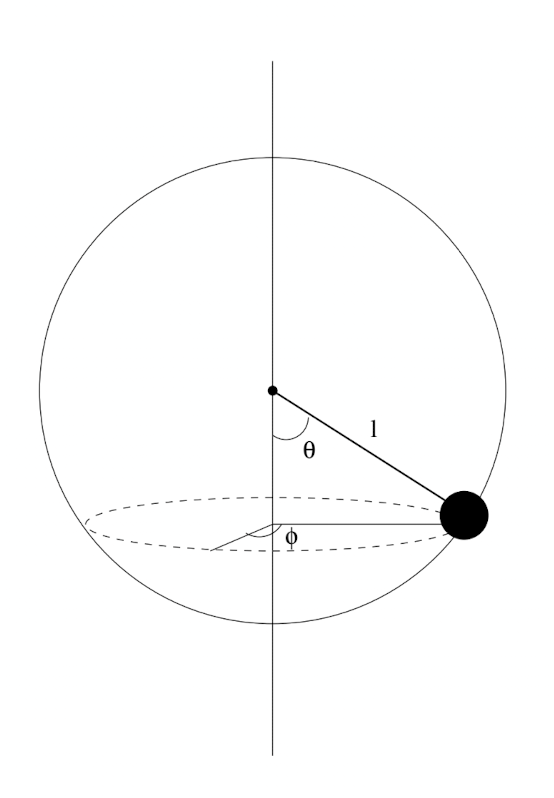
\includegraphics[width=0.4\textwidth]{pendolo_sferico}
  \end{center}
\end{wrapfigure}

Il pendolo sferico pu\`{o} ruotare in tre dimensioni. Il sistema possiede due gradi di libert\`{a} dati dagli angoli $\theta \in [0,\pi)$ e $\phi \in [0,2\pi)$ ed \`{e} soggetto alla forza di gravit\`{a}. Il vincolo del punto materiale \`{e} espresso dalla funzione 
\begin{equation*}
	f = x^2+y^2+z^2 -R^2 = 0
\end{equation*}
e le coordinate cartesiane vengono parametrizzate rispetto al vincolo venendo trasformate in coordinare sferiche 
\begin{equation*}
	\left \{ \begin{array}{l}
		x = R \, cos\phi \, sin\theta \\
		y =R \, sin\phi \, sin \theta \\
		z = -R \, cos \theta
	\end{array} \right.
\end{equation*}
la Lagrangiana del sistema rispetto alle coordinare parametrizzate \`{e} data da 
\begin{equation*}
	\mathcal{L} = \frac{1}{2} m l^2\left(\dot{\theta}^2+\dot{\phi}^2 \sin ^2 \theta\right)+m g l \cos \theta
\end{equation*}
applicando il teorema di Noether rispetto alla trasformazione in coordinate sferiche si ha che la grandezza 
\begin{equation}
	L_0=\frac{\partial L}{\partial \dot{\phi}}=m R^2 \dot{\phi} \sin ^2 \theta
\end{equation}
\`{e} una costante e dunque $\phi$ \`{e} una variabile ciclica del problema. Tale grandezza coincide con il momento angolare lungo la direzione $\phi$. Di conseguenza l' equazione del moto di E-L \`{e} data solo rispetto alla coordinata lagrangiana $\theta$
\begin{equation}
m R^2 \ddot{\theta}=m R^2 \dot{\phi}^2 \sin \theta \cos \theta-m g R \sin \theta
\end{equation}
di conseguenza possiamo andare a definire la Lagrangiana ridotta andando a sostituire
\begin{equation*}
	\dot{\phi} = \frac{L_0}{mR^2sin^2\theta}
\end{equation*}
all'interno dell'equazione dell'energia del sistema ottenendo
\begin{equation}
E(\theta,\dot{\theta})=\underbrace{\frac{1}{2} m R^2 \dot{\theta}^2}_{\text{Termine Cinetico}}+ \underbrace{\frac{L_0}{2 m R^2 \sin ^2 \theta}+m g R \cos \theta}_{\text{Potenziale efficace}}
\end{equation}
di conseguenza la Lagrangiana efficace (o ridotta) si definisce come 
\begin{equation}
	\mathcal{L}_{eff}(\theta ,\dot{\theta}) = \frac{1}{2} m R^2 \dot{\theta}^2 - \frac{L_0}{2 m R^2 \sin ^2 \theta}-m g R \cos \theta
\end{equation}
e le equazioni del moto ridotte assumono la forma \begin{equation}
m R^2 \ddot{\theta}=-\frac{L_0^2 \cos \theta}{m R^2\left(\sin ^3 \theta\right)}-m g R \sin \theta
\end{equation}

\begin{remark}
	Bisogna sostituire $\dot{\phi}$ nell'energia o nelle equazioni del moto. Se si sostituisce direttamente nella Lagrangiana si deriva un equazione simile alla 3.123, ma con un segno meno sbagliato. Questo \`{e} dovuto al fatto che le equazioni di E-L sono derivate assumendo che $\theta$ e $\phi$ siano indipendenti tra loro.
\end{remark}
\noindent Nello studio del moto possiamo formulare due ipotesi:
\begin{itemize}
	\item $L_0 = 0 $: in questo caso l'equazione del modo coincide con quella di un pendolo semplice 
 \begin{equation*}
\ddot{\theta}= - \frac{g}{R}  \sin \theta
\end{equation*}
\item $L_0 \neq 0$: in questo caso abbiamo che 
\begin{equation*}
	mR^2 \ddot{\theta} = - \frac{\partial U_{eff}}{\partial \theta}
\end{equation*}
che coincide con l'equazione 3.123. Di conseguenza per capire il comportamento del sistema studiamo qualitativamente il potenziale efficace.
\end{itemize}

\subsubsection{Studio qualitativo del potenziale efficace per $L_0 \neq 0$}

\noindent Riscriviamo il potenziale efficace come
\begin{equation*}
	U_{eff}(\theta) = \frac{L_0}{2 m R^2 \sin ^2 \theta}+m g R \cos \theta = Bcos\theta + \frac{A}{2sin^2\theta} \quad A,B >0
\end{equation*}
e ne studiamo qualitativamente il comportamento, avremo che $U_{eff}$ possiede due asintoti verticali in $0^+$ e $\pi^{-}$
\begin{equation*}
	\lim_{\theta \rightarrow \theta^+,\pi^{-}} U_{eff} = + \infty 
\end{equation*}
rispettivamente la derivata prima \`{e} data da 
\begin{equation*}
	U_{eff}^{\prime} = -Bsin^4\theta - \frac{Acos\theta}{sin^3\theta}
\end{equation*}
poich\`{e} la funzione \'{e} continua e  possiede due asintoti con lo stesso segno al limite ed \`{e} definita positiva tra essi, ci aspettiamo che sia convessa e dunque esiste un punto di minimo. Per determinarlo studiamo qualitativamente la soluzione di
\begin{equation*}
	sin^4\theta = \frac{A}{B}cos\theta
\end{equation*}
\newpage
\begin{figure}
\centering
\begin{minipage}{.5\textwidth}
  \centering
  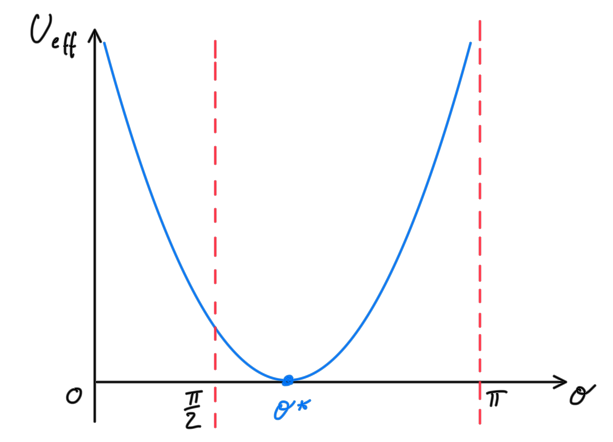
\includegraphics[width=1\linewidth]{potenziale_efficace}
\end{minipage}%
\begin{minipage}{.5\textwidth}
  \centering
  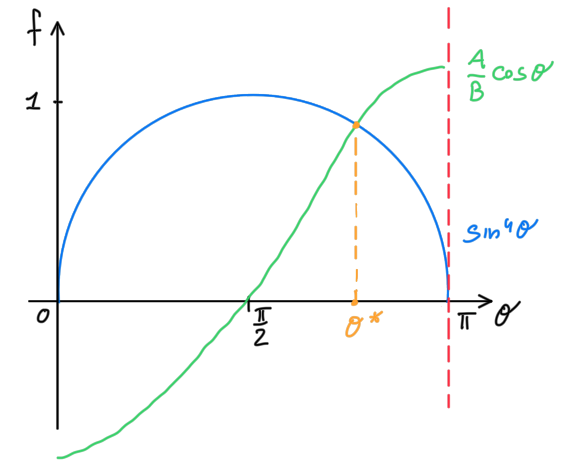
\includegraphics[width=1\linewidth]{solution1}
\end{minipage}
\end{figure}
\noindent dall'immagine soprastante si deduce che esista un punto di minimo $\theta^* \in [\frac{\pi}{2},\pi)$. Se l'energia del sistema coincide con $E = E_{min}$ ovvero $\theta(t) = \theta^* \quad \forall t$ dalle equazioni del moto di ha che 
\begin{equation*}
	\dot{\phi} = \frac{L_0}{mR^2 sin^2\theta^*}
\end{equation*}
dunque essendo $\theta$ costante anche, si dall'equazione precedente abbiamo che il punto materiale si muove di moto circolare uniforme. Se l'energia $E > E_{min}$ si hanno delle traiettorie periodiche. Il cui periodo \`{e} dato da 
\begin{equation}
	T = 2\int_{\theta_{min}}^{{\theta_{max}}} \frac{d\theta}{\sqrt{\frac{2}{mR^2}(E-U_{eff})}}
\end{equation}
Il modolo del pendolo \`{e} periodico rispetto la coordinata $\theta$, ma non \`{e} necessariamente veto che lo sia anche rispetto $\phi$. Di conseguenza possiamo domandarci se il moto complessivo del sistema sia periodico, ovvero se la particella parte da un punto dopo un determinato periodo di tempo ci ritorna ?

\subsubsection{Periodicit\`{a} totale del moto}
\begin{wrapfigure}[5]{r}{0.3\textwidth}
\vspace{-1.2in}
  \begin{center}
    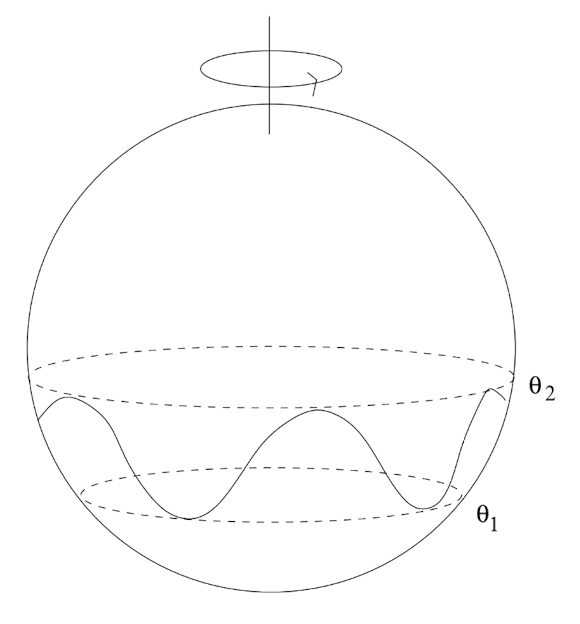
\includegraphics[width=0.4\textwidth]{orbit}
  \end{center}
\end{wrapfigure}
Preso un livello di energia $E > E_{min}$, abbiamo visto che l'angolo $\theta $ pu\`{o} assumere valori solo tra $[\theta_{min},\theta_{max}]$. In mezzo a tali due punti esiste $\theta^*$ rispetto al quale il potenziale efficace $U_{eff}$ \`{e} minimo e rappresenta un orbita stabile. Tale configurazione viene assunta se si bilancia il momento angolare $L_0$ e l'energia E nel modo corretto. 
\newline
\noindent Per studiare la periodicit\`{a} del moto rispetto all'angolo $\phi$ esprimiamo 
\begin{equation}
	\frac{d \phi}{d \theta} = \frac{d \phi}{dt} \frac{dt}{d \theta} = \frac{L_0}{2mR^2sin^2\theta} \left (\frac{d\theta}{dt} \right )^{-1}
\end{equation}
dove 
\begin{equation*}
	\frac{d\theta}{dt} = \frac{2(E-U_{eff})}{mR^2}
\end{equation*}
di conseguenza da 3.125 abbiamo
\begin{equation}
\Delta \phi=2 \int_{\theta_{m, n}}^{\theta_{\max }} \frac{d \varphi}{d \theta} d \theta=2 \int_{\theta_{\min }}^{\theta_{m a x}} \frac{L_0}{m R^2 \sin ^2 \theta} \frac{1}{\left[\frac{2}{m R^2}\left(E-U_{c f f}\right)\right]^{1 / 2}} d \theta
\end{equation}
il moto totale del sistema \`{e} periodico quando 
\begin{equation}
	T = \frac{2 \pi}{\Delta \phi} = \frac{n}{m} \in \mathbb{Q}
\end{equation}

\subsection{Potenziali generalizzati}

Fino a questo punto si \`{e} costruita la teoria Lagrangiana, considerando  solo forze di natura conservativa che possono essere espresse rispetto al potenziale. Come sappiamo dalla meccanica Newtoniana esistono tipi di forze che non dipendono dalla posizione come per esempio l'attrito viscoso, ma dalla velocit\`{a}. Di conseguenza \`{e} necessario costruire una formulazione Lagrangiana che ci permetta di trattare questi tipi di forze.
\newline

\noindent Nel caso in cui si ha un energia potenziale V non conservativa questa prende il nome di \textbf{potenziale generalizzato} se dipende dalle velocit\`{a}

\begin{lemma}
Un potenziale generalizzato V \`{e} al pi\'{u} lineare rispetto alle $\dot{q}_{\alpha}$	
\end{lemma}
\begin{proof}
	Sia $V_{\alpha} = V_{\alpha}(q_{\alpha},\dot{q}_{\alpha},t)$ e ammetta derivate parziali nulle 
\begin{equation*}
\frac{\partial}{\partial \dot{q}_{\alpha}}\left(\frac{\partial V}{\partial \dot{q}_{\beta}}\right)=0
\end{equation*}
allora V \`{e} affine rispetto le $\dot{q}$, ovvero
\begin{equation*}
V=\sum_\alpha A_\alpha(q, t) \dot{q}_{\alpha}-U(q, t)
\end{equation*}
il termine 
\begin{equation*}
\begin{aligned}
Q_\alpha =\frac{d}{d t} \frac{\partial V}{\partial \dot{q}^\alpha}-\frac{\partial V}{\partial q^\alpha} & =\frac{d}{d t} A_\alpha(q, t)-\sum_\beta \frac{\partial A_\beta}{\partial q^\alpha} \dot{q}^\beta+\frac{\partial U}{\partial q^\alpha} \\
& =\sum_\beta \frac{\partial A_{\alpha}}{\partial q^\beta} \dot{q}^\beta+\frac{\partial A_{\alpha}}{\partial t}-\sum_\beta \frac{\partial A_\beta}{\partial q^\alpha} \dot{q}^\beta+\frac{\partial U}{\partial q^\alpha}
\end{aligned}
\end{equation*}
che possiamo riscrivere come 
\begin{equation}
\frac{d}{d t} \frac{\partial V}{\partial \dot{q}^\alpha}-\frac{\partial V}{\partial q^\alpha}=\sum_\beta\left(\frac{\partial A_{\alpha}}{\partial q^\beta}-\frac{\partial A_{\beta}}{\partial q^\alpha}\right) \dot{q}^\beta+\frac{\partial A_{\alpha}}{\partial t} +\frac{\partial U}{\partial q^\alpha}
\end{equation}
dunque $Q_{\alpha}$ dipende linearmente dalle $\dot{q}$.
\end{proof}
\begin{lemma}
	La potenza delle forze \`{e} data da 
	\begin{equation}
\pi=\sum_\alpha^1 Q_\alpha \dot{q}^\alpha=\sum\left(\frac{\partial A_{\alpha}}{\partial t}+\frac{\partial U}{\partial q^\alpha}\right) \dot{q}^\alpha
\end{equation}
dove 
\begin{equation}
\sum_\alpha \sum_\beta\left(\frac{\partial A_{\alpha}}{\partial q^\beta}-\frac{\partial A_{\beta}}{\partial q^\alpha}\right) \dot{q}^\beta \dot{q}^\alpha=0
\end{equation}
\end{lemma}
\subsection{Particella carica in un campo elettromagnetico }
\noindent Si consideri una particella di carica \textit{q} e massa \textit{m} immersa in un campo elettromagnetico $\bm {E}$ e $\bm{B}$, ricordiamo che tali grandezze possono essere riscritte rispetto a un potenziale vettore $\bm{A}(\bm{x},t)$ e un potenziale scalare $\phi(\bm{x},t)$
\begin{equation*}
\mathbf{B}=\nabla \times \mathbf{A} \quad, \quad \mathbf{E}=-\nabla \phi-\frac{1}{c}\frac{\partial \mathbf{A}}{\partial t}
\end{equation*}
la carica \textit{q} sar\`{a} soggetta alla somma della forza di Coulomb e di Lorentz 
\begin{equation*}
	m \ddot{\bm{x}} = q \left [ \bm{E} + \frac{1}{c} \; \dot{x} \times \bm{B}\right ] 
\end{equation*}
che possiamo riscrivere come 
\begin{equation}
m \ddot{x}=-q \nabla \phi-\frac{q}{c} \frac{\partial \bm{A}}{\partial t}+\frac{q}{c}(\bm{\dot{x}} \times (\nabla \times \bm{A}))
\end{equation}
Dimostriamo che dato un \textbf{potenziale generalizzato}
\begin{equation}
U=q \phi-\frac{q}{c}\langle\bm{A}, \bm{\dot{x}}\rangle
\end{equation}
e definita la Lagrangiana 
\begin{equation}
L=\frac{1}{2} m \dot{\mathbf{x}}^2+\frac{q}{c}\langle \bm{\dot{x}},\mathbf{A} \rangle - q \phi
\end{equation}
le equazioni di E-L coincidono con l'espressione 3.128, infatti 
\begin{equation}
\frac{d}{d t}\left(\frac{\partial L}{\partial \dot{\mathbf{x}}}\right)-\frac{\partial L}{\partial \mathbf{x}}=\frac{d}{d t}(m \dot{\mathbf{x}}+\frac{q}{c} \mathbf{A})+q \nabla \phi-\frac{q}{c} \nabla(\dot{\mathbf{x}} \cdot \mathbf{A})=0
\end{equation}
il termine 
\begin{equation*}
	\frac{d\bm{A}}{dt} = \sum_{i} \frac{\partial \bm{A}}{\partial x_i}\dot{x}_{i} + \frac{\partial \bm{A}}{\partial t} 
\end{equation*}
osserviamo che il termine
\begin{equation*}
 B_c = \varepsilon_{cab} \frac{\partial A_b}{\partial x_a} \quad \iff \quad \varepsilon_{avc}B_c = \frac{\partial A_b}{\partial x_a} - \frac{\partial A_a}{\partial r_b}
\end{equation*}
dunque possiamo riscrivere le equazioni del moto di E-L come 
\begin{equation}
m \ddot{r}_a=e E_a+e \epsilon_{a b c} \dot{r}_b B_c
\end{equation}
 che in notazione vettoriale coincidono con 3.128.

\subsubsection{Invarianza rispetto alla trasformazione di Gauge}

Il potenziale scalare e vettore non sono unici. In quanto potremmo fare una trasformazione 
\begin{equation}
\phi \rightarrow \phi-\frac{\partial \chi}{\partial t} \quad, \quad \mathbf{A} \rightarrow \mathbf{A}+\nabla \chi
\end{equation}
e otterremo gli stessi campi $\bm{E}$ e $\bm{B}$ per qualsiasi funzione $\chi$
. Tali trasformazioni prendono il nome di trasformazioni di Gauge. Sotto tali trasformazioni la Lagrangiana non rimane invariata 
\begin{equation}
L \rightarrow L+ \frac{q}{c} \frac{\partial \chi}{\partial t}+ \frac{q}{c} \dot{\mathbf{x}} \cdot \nabla \chi=L+ \frac{q}{c}\frac{d \chi}{d t}
\end{equation}
ma rimangono preservate le equazioni del moto.

